%preamble - package inclusion and set up
\documentclass[12pt,twoside,a4paper,english]{report} %normalt 12pt!!!!
% Select encoding of your inputs
\usepackage[utf8]{inputenc}
% Make latex understand and use the typographic
% rules of the language used in the document.
%\usepackage[danish]{babel}
\usepackage[english]{babel}

% Use the vector font Latin Modern which is going
% to be the default font in latex in the future.
\usepackage{lmodern}
%\usepackage{mathptmx}

% Choose the font encoding
\usepackage[T1]{fontenc}

% Use color in tables
\usepackage[table]{xcolor}
\usepackage{pbox}
\usepackage{tabularx}
\usepackage{array}
\usepackage{multirow}

% Load a colour package
\usepackage{xcolor}
\definecolor{aaublue}{RGB}{33,26,82}  %<--define aaublue
\definecolor{white}{RGB}{255,255,255} %<--define white

% ref stuffz			original position
%\usepackage{cleveref}

% The standard graphics inclusion package
\usepackage{graphicx}

\makeatletter
  \g@addto@macro\@floatboxreset\centering %<--centering all figures
\makeatother

\usepackage{adjustbox}

% Set up how figure and table captions are displayed

\usepackage{float}
\restylefloat{figure}
\usepackage{caption}
\usepackage{subfigure}
\usepackage[subfigure]{tocloft}
\captionsetup
{
  %justification = centering,    %<--centering caption with multiple lines
  %justification = raggedright,  %<-- right alings caption with multiple lines
  justification = justified,  %<-- justify alings (make left and right side equal) caption with multiple lines
  font          = footnotesize, %<--set font size to footnotesize
  labelfont     = bf            %<--bold label (e.g., Figure 3.2) font
}
\captionsetup[subfigure]
{
  justification = centering, %<--centering subfigure caption text
  singlelinecheck=false,
  font = footnotesize        %<--font size for subfigures
} 

% Enable row combination in tables
\usepackage{multirow}

% Make space between table lines and text
\renewcommand{\arraystretch}{1.5}

% Enable commands like \st (strike out) and \hl (high light)
\usepackage{soul}

% Make the standard latex tables look so much better
\usepackage{array,booktabs}

% Enable the use of frames around, e.g., theorems
% The framed package is used in the example environment
\usepackage{framed}
\usepackage{colortbl}
\usepackage{longtable}
\usepackage{xcolor}
\usepackage{textcomp}
\usepackage{indentfirst}
\setlength{\parindent}{1.5cm}
%-------MATHEMATICS---------------------------------
% Defines new environments such as equation,
% align and split 
\usepackage{amsmath}
\usepackage{relsize}
% Adds new math symbols
\usepackage{amssymb}
% Use theorems in your document
% The ntheorem package is also used for the example environment
% When using thmmarks, amsmath must be an option as well. Otherwise \eqref doesn't work anymore.
\usepackage[framed,amsmath,thmmarks]{ntheorem}
\usepackage{xifthen}%<--enables ifthenelse which is used in macros

\usepackage{siunitx} 
\sisetup{decimalsymbol=period}%<--\num{} will swich commas with periods
\sisetup{detect-weight}
%---------------------------------------------------

%-------PAGE LAYOUT---------------------------------
% Change margins, papersize, etc of the document
\usepackage[
  left=25mm,% left margin on an odd page %tidligere 25mm for baade right og left
  right=25mm,% right margin on an odd page
  top=35mm,
  ]{geometry}
  
% Modify how \chapter, \section, etc. look
% The titlesec package is very configureable
\usepackage{titlesec}
\makeatletter
\def\ttl@mkchap@i#1#2#3#4#5#6#7{%
    \ttl@assign\@tempskipa#3\relax\beforetitleunit
    \vspace{\@tempskipa}%<<<<<< REMOVE THE * AFTER \vspace
    \global\@afterindenttrue
    \ifcase#5 \global\@afterindentfalse\fi
    \ttl@assign\@tempskipb#4\relax\aftertitleunit
    \ttl@topmode{\@tempskipb}{%
        \ttl@select{#6}{#1}{#2}{#7}}%
    \ttl@finmarks  % Outside the box!
    \@ifundefined{ttlp@#6}{}{\ttlp@write{#6}}}
\makeatother

\titlespacing{\chapter}{0pt}{0pt}{10pt}
\titlespacing{\section}{0pt}{0pt}{-5pt}
\titlespacing{\subsection}{0pt}{8pt}{-5pt}
\titlespacing{\subsubsection}{0pt}{6pt}{-10pt}

\titleformat*{\section}{\normalfont\Large\bfseries\color{aaublue}}
\titleformat*{\subsection}{\normalfont\large\bfseries\color{aaublue}}
\titleformat*{\subsubsection}{\normalfont\normalsize\bfseries\color{aaublue}}

\usepackage{titlesec, blindtext, color}
%\color{gray75}{gray}{0.75}
\newcommand{\hsp}{\hspace{20pt}}
\titleformat{\chapter}[hang]{\Huge\bfseries}{\thechapter\hsp\textcolor{aaublue}{|}\hsp}{0pt}{\Huge\bfseries}

% Change the headers and footers
\usepackage{fancyhdr}
\setlength{\headheight}{15pt}
\pagestyle{fancy}
\fancyhf{} %delete everything
\renewcommand{\headrulewidth}{0pt} %remove the horizontal line in the header
\fancyhead[RO,LE]{\color{aaublue}\small\nouppercase\leftmark} %even page - chapter title
\fancyhead[LO]{}
\fancyhead[RE]{} 
\fancyhead[CE]{}
\fancyhead[CO]{}
\fancyfoot[RE,LO]{\thepage}
\fancyfoot[LE,RO]{} %page number on all pages
\fancyfoot[CE,CO]{}

% change first page of all chapters header and footer to fancy style
\makeatletter
\let\ps@plain\ps@fancy
\makeatother

% Do not stretch the content of a page. Instead,
% insert white space at the bottom of the page
\raggedbottom

% Enable arithmetics with length. Useful when typesetting the layout.
\usepackage{calc}
%---------------------------------------------------

\usepackage{appendix}

%-------BIBLIOGRAPHY--------------------------------
%setting references (using numbers) and supporting i.a. Chicargo-style:
\usepackage{etex}
\usepackage{etoolbox}
\usepackage{keyval}
\usepackage{ifthen}
\usepackage{url}
\usepackage{csquotes}
\usepackage[backend=bibtex, isbn=false, url=false, eprint=false, doi=false, style=numeric, sorting=none]{biblatex}
\addbibresource{setup/bibliography.bib}
%---------------------------------------------------

%-------MISC----------------------------------------
%%% Enables the use FiXme refferences. Syntax: \fxnote{...} %%%
\usepackage[footnote, draft, english, silent, nomargin]{fixme}		%!!!! DRAFT OR FINAL?!?!?!?!11!! change later!	
%With "final" instead of "draft" an error will ocure for every FiXme under compilation.

%%% allows use of lorem ipsum (generate i.e. pagagraph 1 to 5 with \lipsum[1-5]) %%%
\usepackage{lipsum}

%%% Enables figures with text wrapped tightly around it %%%
\usepackage{wrapfig}

%%% Section debth included in table of contents (1 = down to sections) %%%
\setcounter{tocdepth}{1}

%%% Section debth for numbers (1 = down to sections) %%%
\setcounter{secnumdepth}{2}

\usepackage{tocloft}
\setlength{\cftbeforetoctitleskip}{0 cm}
\renewcommand{\cftpartpresnum}{Part~}
\let\cftoldpartfont\cftpartfont
\renewcommand{\cftpartfont}{\cftoldpartfont\cftpartpresnum}
%---------------------------------------------------

%-------DANSK SPROG---------------------------------

%\addto\captionsdanish{%
%	\renewcommand{\figurename}{figur}%
%	\let\figureautorefname\figurename%
%	\renewcommand{\tablename}{tabel}%
%	\let\tableautorefname\tablename%
%%	\renewcommand{\equationname}{ligning}%
%%	\let\equationautorefname\equationname%
%	\renewcommand{\chaptername}{Kapitel}%
%	\let\chapterautorefname\chaptername%
%	\renewcommand{\partname}{Del}%
%	\let\partautorefname\partname%
%	\renewcommand{\sectionname}{afsnit}%
%	\let\sectionautorefname\sectionname%
%%	\renewcommand{\thesubsection}{underafsnit}%
%%	\let\subsectionautorefname\thesubsection%
%	\renewcommand{\pagename}{side}%
%	\let\pageautorefname\pagename%
%}

%-------HYPERLINKS----------------------------------
% Enable hyperlinks and insert info into the pdf
% file. Hypperref should be loaded as one of the 
% last packages
\usepackage{nameref}
\usepackage{hyperref}
\usepackage{bookmark}
\hypersetup{%
	%pdfpagelabels=true,%
	plainpages=false,%
	pdfauthor={Author(s)},%
	pdftitle={Title},%
	pdfsubject={Subject},%
	bookmarksnumbered=true,%
	colorlinks,%
	citecolor=aaublue,%
	filecolor=aaublue,%
	linkcolor=aaublue,% you should probably change this to black before printing
	urlcolor=aaublue,%
	pdfstartview=FitH%
}

% ref stuffz		new position
\usepackage{cleveref}

\crefname{appsec}{bilag}{bilag}
%---------------------------------------------------



% remove all indentations
\setlength\parindent{0pt}
\parskip 5mm
\usepackage{verbatim}

\definecolor{Gra}{RGB}{230,230,230}

%creates a nice-looking C#-text
\newcommand{\CC}{C\nolinebreak\hspace{-.05em}\raisebox{.3ex}{\scriptsize\text \#} }

%enables multi column lists
\usepackage{multicol}

%enables code-examples
\usepackage{listings}

\definecolor{coolblue}{RGB}{32,95,128}
\definecolor{mygreen}{rgb}{0,0.6,0}
\definecolor{mygray}{rgb}{0.5,0.5,0.5}
\definecolor{mymauve}{rgb}{0.58,0,0.82}
\usepackage{textcomp}
\definecolor{listinggray}{gray}{0.9}
\definecolor{lbcolor}{rgb}{0.9,0.9,0.9}

%for c code
\lstdefinestyle{cstyle}{
  backgroundcolor=\color{lbcolor},
	tabsize=4,
	rulecolor=,
	language=C,
  basicstyle=\scriptsize,
  upquote=true,
  aboveskip={1.5\baselineskip},
  columns=fixed,
  showstringspaces=false,
  extendedchars=true,
  breaklines=true,
  prebreak = \raisebox{0ex}[0ex][0ex]{\ensuremath{\hookleftarrow}},
  frame=single,
  showtabs=false,
  numbers=left,
  captionpos=b,
  numbersep=5pt,
  numberstyle=\tiny\color{mygray},
  showspaces=false,
  showstringspaces=false,
  identifierstyle=\ttfamily,
  keywordstyle=\color[rgb]{0,0,1},
  commentstyle=\color[rgb]{0.133,0.545,0.133},
  stringstyle=\color[rgb]{0.627,0.126,0.941},
}
%for python code
\lstdefinestyle{pythonstyle}{
    backgroundcolor=\color{lbcolor},
    tabsize=4,
    rulecolor=,
    language=python,
    basicstyle=\scriptsize,
    upquote=true,
    aboveskip={1.5\baselineskip},
    columns=fixed,
    showstringspaces=false,
    extendedchars=true,
    breaklines=true,
    prebreak = \raisebox{0ex}[0ex][0ex]{\ensuremath{\hookleftarrow}},
    frame=single,
    showtabs=false,
    numbers=left,
    captionpos=b,
    numbersep=5pt,
    numberstyle=\tiny\color{mygray},
    showspaces=false,
    showstringspaces=false,
    identifierstyle=\ttfamily,
    keywordstyle=\color[rgb]{0,0,1},
    commentstyle=\color[rgb]{0.133,0.545,0.133},
    stringstyle=\color[rgb]{0.627,0.126,0.941},
}
%for matlab code
\lstdefinestyle{matlabstyle}{
    backgroundcolor=\color{lbcolor},
    tabsize=4,
    rulecolor=,
    language=Matlab,
    basicstyle=\scriptsize,
    upquote=true,
    aboveskip={1.5\baselineskip},
    columns=fixed,
    showstringspaces=false,
    extendedchars=true,
    breaklines=true,
    prebreak = \raisebox{0ex}[0ex][0ex]{\ensuremath{\hookleftarrow}},
    frame=single,
    showtabs=false,
    numbers=left,
    captionpos=b,
    numbersep=5pt,
    numberstyle=\tiny\color{mygray},
    showspaces=false,
    showstringspaces=false,
    identifierstyle=\ttfamily,
    keywordstyle=\color[rgb]{0,0,1},
    commentstyle=\color[rgb]{0.133,0.545,0.133},
    stringstyle=\color[rgb]{0.627,0.126,0.941},   
}

%for java code
\lstdefinestyle{javastyle}{
	backgroundcolor=\color{lbcolor},
	tabsize=4,
	rulecolor=,
	language=Java,
	basicstyle=\scriptsize,
	upquote=true,
	aboveskip={1.5\baselineskip},
	columns=fixed,
	showstringspaces=false,
	extendedchars=true,
	breaklines=true,
	prebreak = \raisebox{0ex}[0ex][0ex]{\ensuremath{\hookleftarrow}},
	frame=single,
	showtabs=false,
	numbers=left,
	captionpos=b,
	numbersep=5pt,
	numberstyle=\tiny\color{mygray},
	showspaces=false,
	showstringspaces=false,
	identifierstyle=\ttfamily,
	keywordstyle=\color[rgb]{0,0,1},
	commentstyle=\color[rgb]{0.133,0.545,0.133},
	stringstyle=\color[rgb]{0.627,0.126,0.941},
}

%for inline c, syntax: \cline{ codeHere(); }
\lstdefinestyle{cinline}{
    style=cstyle,
    basicstyle=\small,
}
\newcommand\inlinec[1]{ \lstinline[style=cinline]{#1} }

%for inline python, syntax: \pythonline{ codeHere(); }
\lstdefinestyle{pythoninline}{
    style=pythonstyle,
    basicstyle=\small,
}
\newcommand\inlinepython[1]{ \lstinline[style=pythoninline]{#1} }

%for inline matlab, syntax: \matlabline{ codeHere(); }
\lstdefinestyle{matlabinline}{
    style=matlabstyle,
    basicstyle=\small,
}
\newcommand\inlinematlab[1]{ \lstinline[style=matlabinline]{#1} }

\usepackage{enumitem}
%\usepackage[citestyle=authoryear,natbib=true]{biblatex}

% Figures - TIKZ
\usepackage{tikz}
\usepackage[americanresistors,americaninductors,americancurrents, americanvoltages]{circuitikz}

% Wall of text logo
\newcommand{\walloftextalert}[0]{\includegraphics[width=\textwidth]{walloftext.png}}

\usepackage{pdfpages}
\usepackage{lastpage}
\usepackage{epstopdf}

\setlength{\headheight}{21pt}

\hfuzz=\maxdimen
\tolerance = 10000
\hbadness  = 10000

\usepackage{siunitx}
\graphicspath{{./figures/}}

%macros - please read this file
%Macro for 'where'-enviroment was improved by Andrea and Niels :-)

%-----------UNITS-------------------------------------------
\newcommand{\unit}[1]{&& \left[\si{#1}\right]}
%
%\newcommand{\unit}[1]{[\si{#1}]}            %<<| Use these if you want equations to be
%\newcommand{\eq}[2]{&&\si{#1} &= \si{#2}&&} %<<| centered.. .. will appear scrambled
%                                            %  | from one equation to the next though..
%                                            %  | and does not work with long equations.. :/
%
%-----------------------------------------------------------

%-----------WHERE ENVIRONMENT-------------------------------
\newenvironment{where}{\leavevmode{\parindent=1em\indent} Where:\\}{}
\newcommand{\va}[3]
{
  \begin{tabular}{p{20pt} p{40pt} p{290pt} l}
    & { $#1$ } & { #2 } & \ifthenelse{\isempty{ #3 }}  {}  {[{\si{#3}}]} \\
  \end{tabular}\\
}
%-----------------------------------------------------------

%-----------TikZ SETTINGS-----------------------------------
\tikzset{
  block/.style    = {draw, thick, rectangle,
                     minimum height = 2.1em,
                     minimum width = 1.7em},
  sum/.style      = {draw, circle, inner sep=3pt} %<--Adder
}
%-----------------------------------------------------------


%-----------Fanzy reference SETTINGS------------------------
%Figure references:
\newcommand{\figref}[1]{figure \ref{#1}}

%Figure references after full stop/period:
\newcommand{\Figref}[1]{Figure \ref{#1}}

%Table references:
\newcommand{\tabref}[1]{table \ref{#1}}

%Table references after full stop/period:
\newcommand{\Tabref}[1]{Table \ref{#1}}

%Section references:
\newcommand{\secref}[1]{section \ref{#1}} % on page \pageref{#1}}

%Section references:
\newcommand{\Secref}[1]{Section \ref{#1}} % on page \pageref{#1}}

%Subsection references:
\renewcommand{\subref}[1]{section \ref{#1}} % on page \pageref{#1}}

%Subsection references:
\renewcommand{\Subref}[1]{Section \ref{#1}} % on page \pageref{#1}}

%Appendix references:
\newcommand{\appref}[1]{appendix \ref{#1}} % on page \pageref{#1}}

%Appendix references:
\newcommand{\Appref}[1]{Appendix \ref{#1}} % on page \pageref{#1}}

%chapter references: 
\newcommand{\chapref}[1]{chapter \ref{#1}} % on page \pageref{#1}}

%chapter references: 
\newcommand{\Chapref}[1]{Chapter \ref{#1}} % on page \pageref{#1}}

%Units:
%\newcommand{\unit}[1]{&& \left[\si{#1}\right]}

%Text:
\newcommand{\tx}[1]{\text{#1}}

%Equation references:
%1 equation:
\renewcommand{\eqref}[1]{equation (\ref{#1})}

%-----------------------------------------------------------





\begin{document}       % TIP: If you are using TeXstudio you can open
%\tableofcontents      %      the file by Ctrl+LeftClick on setup/macros.tex
%\pagebreak             %      If the file doesn't exist, you will be asked
					   %      weather or not you want to create it.
%\begin{center}
%	\vspace{5cm}
%	\Huge{Worksheets}
%\end{center}
%\clearpage

%||||||||||||||||||||||||||||||||||||||||||||||||||||||||||||||||
%|||||||                 Example Inputs                  ||||||||
%||||||||||||||||||||||||||||||||||||||||||||||||||||||||||||||||
%|||||||                                                 ||||||||
%			 \input{chapters/aFigureSample.tex}			 %|||||||
%			 \input{chapters/bTableSample.tex} 		     %|||||||
%			 \input{chapters/cEquationSample.tex}		 %|||||||
%			 \input{chapters/dTikzSample.tex}            %|||||||
%			 \input{chapters/eCodeSample.tex}            %|||||||
%|||||||                                                 ||||||||
%||||||||||||||||||||||||||||||||||||||||||||||||||||||||||||||||
%||||||||||||||||||||||||||||||||||||||||||||||||||||||||||||||||


%%% Prereport %%%
		\setlength\cftaftertoctitleskip{2pt}
		\setlength\cftafterloftitleskip{6pt}
		\setlength\cftafterlottitleskip{6pt}
%\selectlanguage{danish}

%%% Frontmatter Settings %%%
		\pagestyle{empty} %disable headers and footers
		\pagenumbering{roman} %use roman page numbering in the frontmatter I II...
	%	\fancyfoot[RE,LO]{18??} %page number on all pages
		\fancyfoot[LE,RO]{\thepage}
		\fancyhead[LE,LO,RE,RO]{}

%%% Introductory Formalities %%%
%\includepdf[pages={1}]{formalities/frontpage.tex}
			\clearpage
\thispagestyle{empty}

\begin{figure}[H]
	\raggedleft
	
\includegraphics[width=0.2\textwidth]{figures/aaulogo-en.png}
\end{figure} 

\vspace{5 cm}

\begin{center}
	\begin{Huge}
		\textbf{Evaluation of Electrotactile Feedback Schemes in a
			Closed-Loop Myoelectric Prosthesis}\\
		\vspace{5 mm}
		Master Thesis \\
		Biomedical Engineering \& Informatics - Spring $2019$\\
		\vspace{3 mm}
	\end{Huge}
	{\Large Project group: $19$gr$10407$} \\
	\vspace{1cm}
	\large{Christian Korfitz Mortensen, Martin Alexander Garenfeld}
\end{center}
\vspace*{\fill}

\begin{center}
	\line(1,0){400}
\end{center}

%\newpage
%
%\large{\textbf{Project period:}\\
%P7, Autumn 2017\\
%01/08/2017 - 20/12/2017\\
%
%\textbf{Project group:}\\
%17gr7404\\} %\fxnote{Input group number}
%
%
%\begin{center}
%	\Large{\textbf{Collaborators:}\\
%		\vspace{1.5cm}
%	\rule{10cm}{1pt}\\
%	Irene Uriarte \\
%	
%	\rule{10cm}{1pt}\\
%	Martin Alexander Garenfeld \\
%	
%	\rule{10cm}{1pt}\\
%	Oliver Thomsen Damsgaard \\
%	
%	\rule{10cm}{1pt}\\
%	Simon Bruun \\}
%\end{center}
%
%
%
%\large{\textbf{Supervisors:}\\
%Strahinja Dosen \\
%Jakob Lund Dideriksen \\
%Lotte N.S. Andreasen Struijk} \\
%\\
\newpage
			% <--- the frontpage
			\pagestyle{fancy}
%{\small
\strut\vfill % push the content to the bottom of the page
\noindent Copyright \copyright{} Aalborg University 2015\par
\vspace{0.2cm}

\noindent This report is compiled in \LaTeX, originally developed by Leslie Lamport, based on Donald Knuth's \TeX. The main text is written in \emph{Latin Modern} pt 12, designed by Bogusław Jackowski and Janusz M. Nowacki. 
%The document is compiled via the website \url{www.overleaf.com}, an online collaborative based \LaTeX-editor with instant preview, which enables multiple persons to edit the document simultaneously.
Flowcharts and diagrams are made using Microsoft Visio. 
\clearpage
			%\begin{document} 
\thispagestyle{empty}
\begin{titlepage}
	\begin{nopagebreak}
		{\samepage 
			
			\begin{tabular}{r}
				\parbox{\textwidth}{  \raisebox{-15mm}{
\includegraphics[height=3cm]{figures/aaulogo-en.png}}
					\hfill \hspace{2cm} \parbox{8cm}{\begin{tabular}{l} %4.90
							{\small \textbf{\textcolor{aaublue}{{3\textsuperscript{rd} Semester, Project}}}}\\
							{\small \textbf{\textcolor{aaublue}{School of Medicine and Health}}}\\
							%{\small \textbf{\textcolor{aaublue}{Communication Technologies}}}\\ 
							{\small \textbf{\textcolor{aaublue}{Biomedical Engineering and Informatics}}}\\
							{\small \textcolor{aaublue}{Fredrik Bajers Vej 7A}} \\
							{\small \textcolor{aaublue}{9220 Aalborg}} \\
							%{\small \textcolor{aaublue}{\emph{http://www.sict.aau.dk/electronics-and-it}}}
				\end{tabular}}}
			\end{tabular}
			
			\begin{tabular}{cc}
				\parbox{7cm}{
					
					\textbf{Title:}
					
					Does Task-related FMRI Preprocessing Need a FIX? \\ 
					
					\textbf{Theme:}
					
					\small{
						Applied Biomedical Engineering and Informatics\\
					}
					
					
					\parbox{8cm}{
						
						
						\textbf{Project period:}\\
						P3, Fall 2018\\
						01/09/2018 - 20/12/2018\\
						
						\textbf{Project group:}\\
						18gr9411\\ %\fxnote{Input group number}
						
						\textbf{Participants:}\\
						Christian Korfitz Mortensen\\
						Martin Alexander Garenfeld\\
						
						
						
						\textbf{Supervisors:}\\
						Robert Coghill\\
						Marie-Eve Hoeppli\\
						Carsten Dahl Mørch\\
						
					}\\
					\\
					\\
					\textbf{Pages:} 83\\
					\textbf{Appendix:} 13 \\
					%\textbf{Ekstra:} For projektkode: Se forord\\ %eks. en CD eller USB
					\textbf{Handed in:} 19/12/2018\\
					\\
					\textit{The content of this report is freely available, but publication (with reference) may only be done with
						agreement with the authors.}
					\vfill } &
				\parbox{7cm}{
					\vspace{-.55cm}
					\hfill
					\begin{tabular}{l}
						{\textbf{Abstract:}} \\
						\fbox{
							\parbox{8.5cm}{\bigskip
								{\vfill{\small The implementation of intuitive and meaningful proprioceptive feedback of myoelectric prosthetic states is an important aspect in enhancing embodiment and user satisfaction, hence lowering the demand for visual attention for prosthetic control in everyday tasks. Therefore, two different configurations for conveying position state information of wrist rotation and hand aperture through electrotactile stimulation were developed and evaluated in a simulated closed-loop prosthesis. A spatially-based configuration was made conveying information by changing the activation of pads in an electrode array placed circumferentially around the non-dominant arm. The other scheme was amplitude-based and used various levels of amplitude from specific electrode pads to convey information of the position state of the prosthesis. 14 able-bodied subjects were evaluated through a Fitts' Law inspired target reaching test following a minimal training session.
The amplitude-based and spatially-based configurations yielded mean completion rates of 93 \% $\boldsymbol{\pm}$ 6 \% and 87 \% $\boldsymbol{\pm}$ 11 \%, respectively. The amplitude feedback configuration yielded a slightly higher completion rate (p = 0.044) than the spatially-based and was also preferred by 64 \% of the subjects. However, with such high completion rates both schemes can be regarded intuitive and was subjectively reported to be useful and easily comprehensible. This manifests that both developed feedback configurations allow subjects to perceive two feedback variables at the same time, despite being implemented in a compact stimulation interface.
										\bigskip}}
						}}
				\end{tabular}}
		\end{tabular}} %\vspace{1cm}
		
		
		%\centering
		%\textit{Offentliggørelse af rapportens indhold, med kildeangivelse, må kun ske efter aftale med forfatterne.}\\
		
	\end{nopagebreak}
\end{titlepage}
%\end{document} 			 % <--- the titlesheet - contains the synopsis!!
%%% Preface %%%
			\cleardoublepage
			
%			The implementation of intuitive and meaningful proprioceptive feedback of myoelectric prosthetic states is an important aspect in enhancing embodiment and user satisfaction, hence lowering the demand for visual attention for prosthetic control in everyday tasks. Therefore, two different configurations for conveying position state information of wrist rotation and hand aperture through electrotactile stimulation were developed and evaluated in a simulated closed-loop prosthesis. A spatially-based configuration was made conveying information by changing the activation of pads in an electrode array placed circumferentially around the non-dominant arm. The other scheme was amplitude-based and used various levels of amplitude from specific electrode pads to convey information of the position state of the prosthesis. 14 able-bodied subjects were evaluated through a Fitts' Law inspired target reaching test following a minimal training session.
The amplitude-based and spatially-based configurations yielded mean completion rates of 93 \% $\boldsymbol{\pm}$ 6 \% and 87 \% $\boldsymbol{\pm}$ 11 \%, respectively. The amplitude feedback configuration yielded a slightly higher completion rate (p = 0.044) than the spatially-based and was also preferred by 64 \% of the subjects. However, with such high completion rates both schemes can be regarded intuitive and was subjectively reported to be useful and easily comprehensible. This manifests that both developed feedback configurations allow subjects to perceive two feedback variables at the same time, despite being implemented in a compact stimulation interface.			 % <--- this is the abstract!!
\clearpage
			\chapter*{Preface}				% <--- the preface
%
%\input{contents/bBackground/title.tex}
\clearpage
			\pdfbookmark[0]{Table of Contents}{label: tableOfCentents}
			\tableofcontents
			\cleardoublepage


%%% Mainmatter Settings %%%
\pagenumbering{arabic} %use arabic page numbering in the mainmatter
\fancyhf{}
\fancyfoot[C]{\thepage} %\text{ of} \pageref{LastPage}			% ADD LABLE{LASTPAGE} TO LAST PAGE !!
\fancyfoot[RE,LO]{19gr10407}																								   %
\fancyhead[RE,LO]{}																												%% } consider fancyfoots
\fancyhead[RE,LO]{\color{aaublue}\small\nouppercase\leftmark} %even page - chapter title %
\pagestyle{fancy}


%---------------------------INPUTS-------------------------------

\part{Paper}

\chapter{Introduction}

The loss of an upper limb can be incredibly traumatic and life changing event with the consequence of a significantly reduced quality of life due to restrictions in function, sensation and appearance \cite{Schofield2014,Ostlie2011}. The loss is additionally linked to multiple mental health disorders \cite{Ostlie2011}.
In an effort to restore pre-trauma functionality, prosthetics of various functionality and complexity have been introduced to replace the missing limb \cite{Geethanjali2016}. However, despite advancements in prosthetic technologies only 50 $\percent$ to 60 $\percent$ of hand amputees wear a prosthetic device \cite{Stephens-Fripp2018}. An explanation for the low user satisfaction should be found in the lack of exteroceptive and proprioceptive feedback provided by commercially available devices \cite{Peerdeman2011}. Presently, merely one device (VINCENT evolution 2, Vincent Systems Gmbh, DE), is commercially available providing the user with feedback information of grasping force, through a feedback interface \cite{Systems2005}. \\    
The missing sensory feedback can cause the prosthetic hand to feel more unnatural and awkward \cite{Pamungkas2015}, thus the user solely have visual feedback to rely on \cite{Stephens-Fripp2018,Pamungkas2015}, which prosthetic user have shown a strong desire to decrease \cite{Atkins1996}. In a survey by Peerdeman et al. \cite{Peerdeman2011} it was found that secondly to providing proportional grasp force feedback, providing positional feedback was of highest priority. Visual independence can be achieved by providing the user with proprioceptive information through somatosensory feedback, possibly facilitating the prosthetic device to be adopted by the user as an integrated part of their body, enhancing the feeling of embodiment and restoring the once physiologically closed loop \cite{Stephens-Fripp2018,Xu2016,Strbac2016,Geng2012}. \\
Various means of recreating the sensory feedback has been sought through either invasive and non-invasive approaches translating information from sensors in the prosthesis to new sensory sites. Invasive methods, termed somatotopically feedback aims to recreate the prior sensory experience by directly stimulating specific nerves in the residual limb \cite{Schofield2014,Stephens-Fripp2018}.
Substitutionary feedback can either be modality matched using pressure as a substitute for grasp force \cite{Godfrey2017} or non modality matched via vibration for grasp force \cite{Ninu2014,Nabeel2016}.
As electrotactile feedback offers modulating multiple parameters such as pulse width, amplitude and frequency to convey feedback information along with the possibility of using multiple feedback channels it seems ideal to utilize these perks for proprioceptive sensory feedback of the multi degree of freedom prosthetic state.  

electrotactile feedback schemes

Based on the current work it would reasonable to investigate which types of electrotactile feedback is perceived more intuitive when conveying proprioceptive sensory feedback of the current prosthetic state. In this study we will present two different stimulation to convey the before mentioned information; one based on activation of differently spatially located electrode pads, and another based on delivering different levels of amplitude.      


 


\part{Worksheets}
\chapter{Background} \label{backback}
The background chapter will outline the considerations that needs to be made when testing the usability of sensory feedback configurations in combination with myoelectric prosthetic control. The feedback will be given based on which motion state a pattern recognition controlled prosthesis is in. \\ 
The main idea behind myoelectric prosthetic control is to translate recorded muscle signals (EMG signals) into a motion performed by the prosthesis. A pattern recognition model can be taught to differentiate between a set of movement classes. When receiving a segmented part of a EMG signal it then decides upon which movement class that most likely is being performed. In combination with the elicited muscle contraction level, this is used as input in the control system and the prosthesis should perform a corresponding motion. \cite{Guanglin2010} In a closed loop prosthesis, the motion state the prosthesis is in can be coded to be equivalent to a certain sensory feedback. The should enable the user to interpret the sensory feedback and use as additional information to visual feedback about the prosthesis' state. \cite{Strbac2016} A closed loop prosthesis iteration can be seen in \figref{fig:closed_loop_pros}. \\
Regarding control the background chapter will explain the following: generation of EMG signals, data acquisition, data processing, pattern recognition and proportional control. Regarding sensory feedback the following will be explained: prior investigations on sensory feedback, types of sensory feedback and sensory feedback configurations. 

\begin{figure}[H]                 
	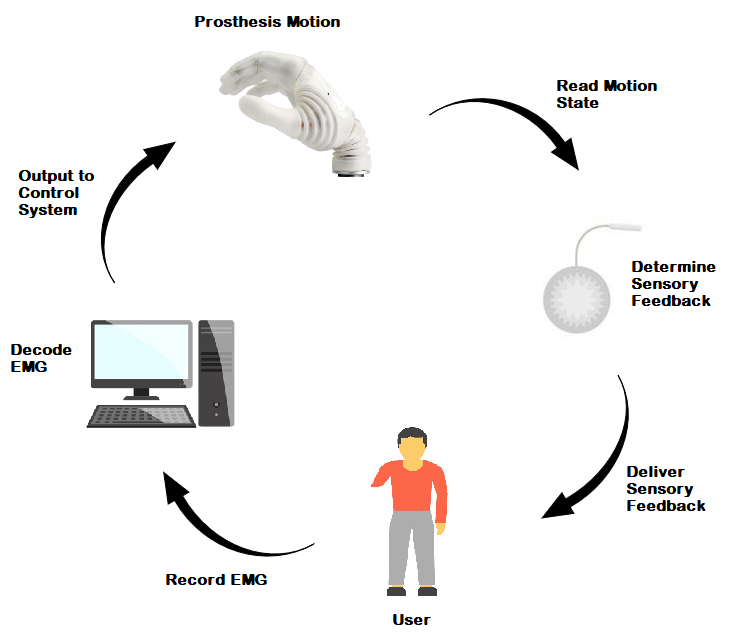
\includegraphics[width=.65\textwidth]{figures/closed_loop_pros}  
	\caption{The figure shows the stages of a closed loop prosthesis. First, EMG signals are recorded from the user. The signals are decoded and an output is relayed to the control system, which is used for the prosthesis to perform a motion. The motion state is then read and sensory feedback is delivered to the user regarding which motion state the prosthesis is in.}
	\label{fig:closed_loop_pros} 
\end{figure}
\section{Sensory Feedback Stimulation} \label{SFS}

It is recognized that vision alone does not provide a sufficient amount information to achieve efficient daily life use of a prosthetic device, as the use requires full visual attention. In the effort of regaining the cutaneous sensations previously felt by the lost limb of a transradial amputee, stimulations of various sorts can be applied on the skin of the remaining stump. These stimulations mimic the information sensed by the lost limb by activating cutaneous receptors. It has been shown both in the acute phase and long term that providing the amputee with sensory feedback can reorganize neurological pathways or even recover original pathways during motor tasks, when trained amply. \cite{Pino2009} \\
Hence, efforts have been put in investigating methods of providing proprioceptive and exteroceptive information of e.g. grasp strength and position state through the means of artificial stimulation. \cite{Schofield2014,Stephens-Fripp2018} Presently, there are multiple ways of providing the user with a variety of sensory feedback. These can be divided into three categories: somatotopical feedback, modality-matched feedback and substitution feedback. \cite{Schofield2014} \\
This section will present general concepts in sensory feedback stimulation and give a brief overview of the types of sensory feedback in order to give insight in the possibilities and eventual disadvantages when providing the user of a prosthetic device with feedback.

\subsection{Somatotopical Feedback}

Somatotopical feedback aims to provide the user with a sensory experience which is perceived as natural as what was felt by their missing limb, both in location and sensation. To achieve such an experience, somatotopical feedback uses invasive approaches by making use of invasive neural electrodes and targeted reinnervation. The former is known as peripheral nerve stimulation and relies on the invasive neural electrodes being interfaced with the original neural pathways preserved proximally on the residual limb. Currently, two different types of electrodes have been exploited: one where a cuff is placed around a nerve fascicle and another where an electrode is implanted into the nerve fiber. But to this date, none of these methods have been comprehensively studied. Targeted reinnervation also enables the possibility of stimulating the original neural pathways from the missing limb. The corresponding sensory afferents are relocated to innervate new sites which can selectively be chosen and stimulated by non-invasive tactors. Somatotopically-matched feedback is hypothesized to reduce the users cognitive burden due to its naturalness, facilitating increased compliance and less cognitive attention. \cite{Schofield2014}  

\subsection{Modality-Matched Feedback}

In modality-matched feedback, the type of sensory experience which would have been felt by the missing limb is communicated to the user at another site. For instance, when pressure is felt in the palm of a prosthetic hand by pressure sensors, a proportional amount of pressure is delivered to the user somewhere on the skin e.g. on the residual limb. Thus, the sensation is not matched in location, but only in sensation. Mechanotactile feedback which conveys pressure information is utilized by the use of e.g. pressure cuffs or servomotors. These types of tactors are very useful for modality-matched feedback, but have a disadvantage by being more power consuming and less practical compared to other stimulation types. \cite{Schofield2014,Antfolk2018} 

\subsection{Substitution Feedback} \label{senssub}

Substitution feedback methods convey sensory information without regarding the type of sensation and location which would have been felt by the missing limb. Thereby, the sensory information is said to be non-physiologically representative. The feedback methods are often straightforward to implement, but demands a greater amount of user adaption to interpret what the feedback information represents. Often used methods for substitution feedback are vibrotactile and electrotactile feedback. \cite{Schofield2014,Antfolk2018}     

\subsubsection{Vibrotactile Stimulation}

Vibrotactile stimulation utilizes small mechanical vibrators to convey information to a selected area of the skin which activates cutaneous mechanoreceptors. This method is mostly used to transfer tactile information in prosthetic grasping tasks. \cite{Schofield2014} A recognizable sensation is evoked using frequencies between 10 and 500 Hz. The sensory threshold varies between users and location, resulting in the need for specific user threshold calibration. \cite{Antfolk2018}  


\subsubsection{Electrotactile Stimulation} \label{E-stim}

In electrotactile feedback a sensation is achieved by stimulating the primary myelinated afferent nerves with an electrical current. The sensation which the stimulation invokes has been reported to be tingling, prickling, itching, buzzing, physically touching and/or burning. \cite{Schofield2014} Electrotactile stimulation rely on small and lightweight electrodes to provide the electrical stimulation. When compared to other feedback methods as vibrational and pressure stimulation, which depend on heavier actuators and moving parts to provide the feedback, this property can be seen as an advantage as prosthetic users strongly desire lightweight systems \cite{Stephens-Fripp2018,Benz2016}. Furthermore, through the use of electrotactile stimulation, multiple factors such as amplitude, pulse width, frequency and location of the stimulation can be controlled facilitating development of agile feedback schemes. This enables the possibility of varying the perceived feedback as either vibration, tapping or touch by modulating the signal waveform. The downside of using electrodes is the requirement for recalibration of sensory thresholds, pulse width and frequency to reproduce the same perceived stimulation every time the electrodes are placed on the user. In addition, interference between electrodes used for stimulation and recording have been found to result in noise in recorded EMG signal used for myoelectric control. However, concentric electrodes are able to limit the interference by limiting the spread of current. Concentric electrodes have also been found to increase localization and perceptibility of the induced stimuli. \cite{Schofield2014,Stephens-Fripp2018,Antfolk2018} 







%Prosthetic users have also shown a strong desire to decrease the need for visual attention to perform functions
\section{State of Art in Electrotactile Feedback} \label{SoA}

\Secref{SFS} presented different types of sensory feedback from which the choice of stimulation in this project can be drawn upon. Somatotopically might restore the most natural sensations, but is also the most complicated. Modality matching the feedback should instead be sought, however present tactors are larger and more power consuming than electrodes uses in electrotactile feedback. Furthermore, the dimensions of electrodes facilitates easier integration with the prosthesis as these can be placed inside the socket, along with electrodes used for acquisition. However, this requires that a solution for leakage current is found. Modulating pulse width, frequency and amplitude in electrotactile feedback gives more possibilities for conveying complex tactile information. Therefore, the state of art methods using electrotactile sensory feedback in the current literature have been reviewed and will presented to ensure that the later derived feedback schemes extends recent evidence. \\
Multiple studies have investigated the use of electrotactile feedback regarding both how distinguishable sensations are evoked and how to convey sensory feedback in different coding schemes for improving myoelectric prosthetic control \cite{Stephens-Fripp2018}. 
In 2015, Shi and Shen \cite{Shi2015} investigated how subjects would perceive the effects of varying amplitude, frequency and pulse width of an electrical stimulation in various combinations. Results showed that appropriate sensations from electrical stimulation would be achieved by varying amplitude from 0.3 mA to 3 mA, pulse width from 0.1 ms to 20 ms and frequency from 40 Hz to 70 Hz. Furthermore, varying these ranges properly would make it possible to have proportionally increased stimulation grades felt by the subject. Additionally, the authors stated the importance of electrode size, as stimulation through to big or to small electrode diameters could result in sensations of pain or discomfort. \cite{Shi2015} \\         
Several studies \cite{Pamungkas2015,Xu2016,Jorgovanovic2014,Isakovic2016} using electrical stimulation have investigated its use in conveying grasping force/pressure feedback. Jorgovanovic et al.\cite{Jorgovanovic2014} investigated users' recognition of grip strength, when controlling a joystick controlled robotic hand, through varying the pulse width and keeping the frequency and intensity constant at 100 Hz and 3 mA, respectively. Results showed that providing electrotactile feedback improved the users' ability to move objects with the robotic hand. \cite{Jorgovanovic2014} Similar result were found by Isakovic et al. \cite{Isakovic2016}, who also showed that electrotactile feedback supported a faster learning than no feedback in grasp force control, and that electrotactile feedback might facilitate short-term learning. \\ 
A study by Xu et al. \cite{Xu2016} tested and evaluated different types of pressure and slip information feedback through electrotactile stimulation and compared this to visual feedback and no feedback. The study recruited 12 subjects, 6 able bodied, and provided electrotactile feedback by keeping the intensity and frequency constant and then varying the pulse width between 0 $\mu s$ and 500 $\mu s$ indicating changes in grasp force. In this case, visual feedback was found to outperform electrotactile feedback. \cite{Xu2016} \\
Pamumgkas et al. \cite{Pamungkas2015} also tested the use of electrotactile feedback to convey information from pressure sensors located in a robotic had. Their setup used six feedback channels corresponding to a pressure sensor in each of the fingers and one in the palm. Pressure information in the sensors were given in three discretized frequency levels of 100 Hz, 60 Hz and 30 Hz for the fingers and 20 Hz for the palm. Reported results stated that the subjects learned how to appropriately use the feedback when picking up objects of various sizes. Furthermore, the subjects reported that they preferred having electrotactile feedback accompanied by visual feedback opposed to only having visual feedback. \cite{Pamungkas2015} 
The purpose of restoring the sensation that would be experienced by touch of the skin has also been pursued in more elaborate efforts through artificial skin \cite{Hartmann2014,Franceschi2015}. In these cases, a grid of 64 pressure sensors were used to translate information of touch into 32 electrotactile electrodes placed on the arm of the subjects. \\
The use of electrotactile feedback has proven useful in cases of restoring the haptic feedback through pressure sensors on a prosthetic hand or by the touch on artificial skin. However, the possibilities of electrotactile feedback have also been investigated in the case of improving prosthetic control. In 2016, Strbac et al. \cite{Strbac2016} presented a novel electrotactile feedback stimulation system, which could be used to convey information about the current state of a multi-DoF prosthesis. The system comprised of four different dynamic stimulation patters communicating the states of four different DoF's through a 16 multi-pad array electrode, possibly restoring both proprioception and force. The state of the three of the DoF's were communicated by altering the electrodes activated in patterned fashion and the fourth DoF by modulating the stimulation frequency. Tests of the stimulation design showed that six amputees were able to recognize the four DoF's with an average accuracy of 86 \percent. \cite{Strbac2016}   \\
In summary most studies have focused on using electrotactile feedback for exteroceptive means while only \cite{Strbac2016} have investigated its use for proprioceptive feedback. However, their results encourage further investigation into how electrotactile feedback can be utilized for providing meaningful proprioceptive feedback.  

\subsection{Sensory Adaptation in Electrotactile Feedback}

Before implementing a electrotactile feedback interface, it is important to consider the effect electric stimulation might impose on the sensory system. \\
Adaption is defined as a changing sensory response to a constant stimulus, and all sensory systems have shown adaptive tendencies. This could result in unreliable effects during prolonged electric stimulation. Hence, it is crucial to consider stimulation parameters which reduce adaption. Sensory adaption usually occurs within minutes, and reaches a maximum after 15 min. Furthermore, the adaption rate is related to the stimulation amplitude as adaption occurs faster when closer to the pain threshold. Low frequencies (<10 Hz) show less adaption compared to higher frequencies (>1000 Hz). The adaption response is found to be exponential in decay and recovery. \cite{Buma2007,Szeto1982} 
However, sensory adaptation can be overcome by using intermittent stimulation, and preferably, stimulation interfaces should consider conveying feedback information through diversified patterns \cite{Szeto1982,Dosen2016}. \\
Developed feedback schemes should consider using as low amplitudes as possible to reduce the rate of sensory adaption. Furthermore, continuously changing the site of stimulation should also facilitate less adaption. 




\section{Closing the Loop}

The loss a limp does not only result in a loss of motor function, sensory function is also impaired. Providing an amputee with a prosthetic device, which does not provide sensory feedback, only restores one half of the one closed limb control loop. To close the loop the prosthetic device needs to contain proprioceptive and exteroceptive sensors, which recorded information needs to be conveyed to the amputee in a intuitive and meaningful way \cite{Markovic2018}. This can be achieved using the before mentioned methods of sensory substitution \cite{Schweisfurth2016}. \\
Closing the loop is a well recognized need of prosthetic users and might improve easiness of use and embodiment, possibly lowering rejection rates. Furthermore, the need for visual attention to correct prosthetic movement would be lowered. \cite{Strbac2016} However, the advantages of closing the loop by providing sensory substitution feedback have been contradictory \cite{Jorgovanovic2014}. In 2008 Cipriani et al. \cite{Cipriani2008} investigated the use of vibroctacile feedback for improving grasp in a prosthetic and did not find any improvement using providing the sensory feedback. Later finding by Witteveen et al. \cite{Witteveen2012} disproved this as they found providing information of grasp force and slip through vibrotactile feedback improved a virtual grasping task. \\
Even though most studies find closing the loop by providing sensory feedback helpful (review by Stephens-Fripp et al.) \cite{Stephens-Fripp2018}, currently one device, the VINCENT evolution 2 (Vincent Systems Gmbh, DE) is commercially available conveying grasp force feedback \cite{Systems2005}.  
Addtionally, closed loop control systems bypassing human interaction have also been investigated and implemented by commercial manufacturers i.e. Otto Bock and RSL steeper. Actuators are made to autonomously adjust grip force based on sensor located in the prosthetic hand. \cite{Xu2016} Such an approach might improve reliability of the prosthesis, but does not provide proprioceptive and exteroceptive to the user thus not promoting embodiment.  





\input{contents/Background/specs_Max.tex}
\section{Electromyography}

The control of a myoelectric prosthesis is based on recorded myoelectric signals. \cite{Geethanjali2016}  Enabling the use of myoelectric signals for control of functional prosthetics requires a theoretical background knowledge of the signals origin and how it can be acquired. The following section will describe myoelectric signals and how they are acquired through the acquisition method of EMG.   

The process of executing a voluntary movement can be explained through electric potentials and the excitability of skeletal muscle fibers. The nerve impulse carrying excitation information of a voluntary muscle contraction will travel from the motor cortex down the spinal cord to a alpha motor neuron. The alpha motor neuron will activate and direct a nerve impulse along its axon to multiple motor endplates, which each innervate a muscle fiber. The motor neuron and the muscle fibers it innervates is in collection called a motor unit. \cite{Turker2013} 

The nerve impulse initiates the release of neurotransmitters forming an endplate potential. The muscle fibers consist of muscle cells, which each are surrounded by a semi-permeable membrane. The resting potential over the membrane is held at a equilibrium, typically at -80 mV to -90 mV, by ion pumps, which passively and actively control the flow of ions through the membrane. The release of neurotransmitters affects the flow through the ion pumps resulting in a greater influx of Na$^+$. This results in a depolarization of the cell membrane. However, only if the influx of Na$^+$ is great enough to create a depolarization surpassing a certain threshold, an action potential is formed. The action potential is characterized by the cell membrane potential, which changes from around -80 mV to +30 mV. %After the depolarization a repolarization phase occurs and is followed by a hyperpolatization period, restoring the resting potential. 
The created action potential will propagate in both directions on the surface of the muscle fiber. This process happens across all muscle fibers in a motor unit. The action potential is also known as a motor unit action potential (MUAP), and it is the superposition of multiple MUAPs that is recorded through surface EMG. The action potential is still measurable on the skin surface, however, some limitations in surface EMG are that the recording is restricted to superficial muscles, that the amplitude of the EMG signal is affected by the depth of subcutaneous tissue and that the distinguishability of MUAP's from adjacent muscles is unreliable. \cite{Turker2013,Martini2012} 

Acquisition of EMG signal can either be carried out through surface EMG or intramuscular EMG. The latter measures MUAPs through needles inserted into the muscle and can and collect MUAPs from single muscle fibers individually. Surface EMG is acquired through electrodes on the skin surface. \cite{Cram2012}  Using surface EMG requires preparation of the skin surface to minimize impedance and maximize skin contact. Hence, the skin should be clean and dry before electrode placement. To further minimize skin-electrode impedance removal of excess body hair or flaky skin and cleansing the area using alcohol swabs should be considered. \cite{Turker2013,Cram2012} In this project, MUAPs will be recorded through surface EMG. An example of a surface EMG recording of two different movements (pronation and supination of the wrist) can be seen in \figref{fig:Emg_rot}. Here, the surface electrodes are placed at the circumference of the forearm of the subject. It can be seen that some electrode channels are more or less active when comparing the two movements. This corresponds to different muscles being more or less contracted depending on which movement that is performed. This facilitates the distinguishability the recognition of which movement is being performed. A prerequisite for this to work is that the electrode placement must be identical throughout the recording. If not, the activation of the various channels shifts spatially, and the accuracy of the trained recognition system might be decreased.

\begin{figure}[H]                 
	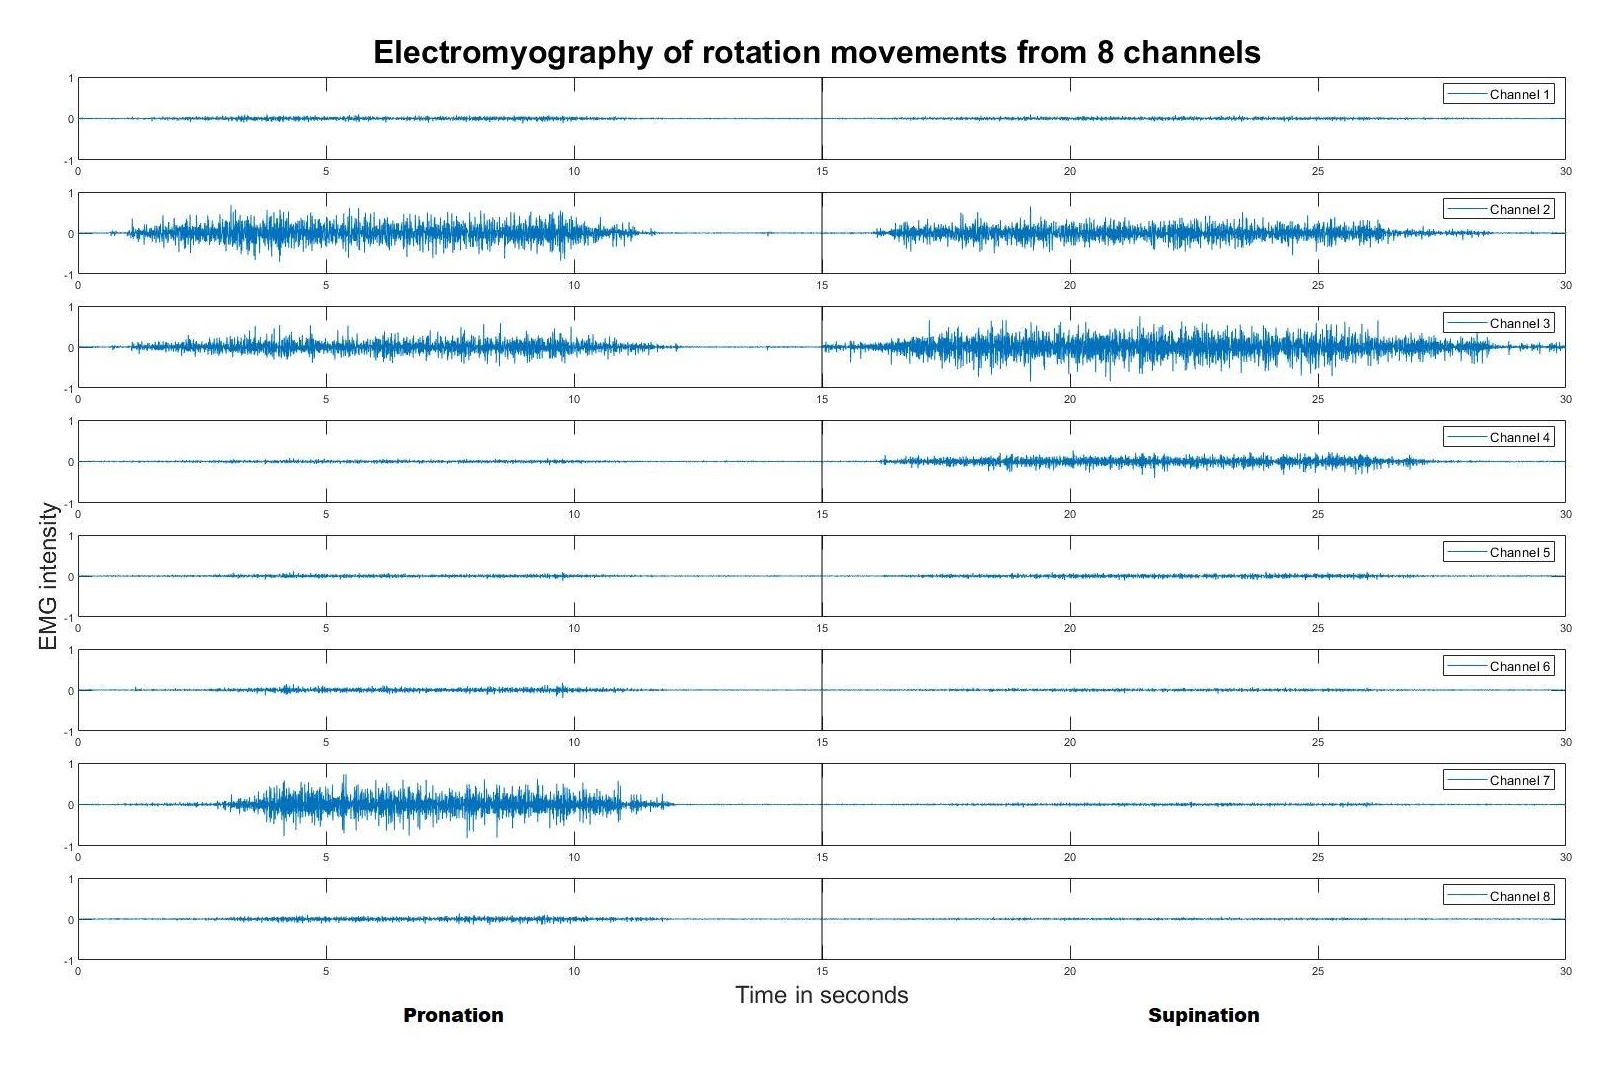
\includegraphics[width=1\textwidth]{figures/Emg_rot}  
	\caption{Illustration of an eight electrode channel surface EMG of the forearm during pronation (left side) and supination (right side) of the wrist. The recording was acquired using the Myo Armband, see \figref{fig:MYB}. The 4th channel was placed on the thickest part of the forearm centrally on the anterior side, when using a pronated arm as reference position, with the horizontal LED light faced laterally towards the wrist.}
	\label{fig:Emg_rot} 
\end{figure}

%surface and iemg emg             

\subsection{Data Acquisition} \label{sec:MYO}
Before a user can utilize a myoelectric prosthesis the control system needs to be taught how certain movements look like represented as EMG signals. This process is called training the control system. The acquisition of training data from the user is therefore the first step in training the control system.

In the acquisition of EMG signals, the Myo Armband (MYB) from Thalmic Labs will be used. It contains eight dry stainless-steel electrode channels embedded inside the armband. The advantage of using dry electrodes is that they do not need to be disposed after use, in contrary to conventional gel electrodes. Thus, the MYB can be reused for all subjects participating in the project, which enables less time consuming experiments. An additional usability advantage is that it communicates wirelessly to external devices via Bluetooth 4.0, leaving no loose wires to possibly limit mobility or distort connection. \cite{Myoarmband2013} 

The MYB acquires EMG signals in an 8-bit resolution. Instead of acquiring the signal in millivolts, the output is scaled to decimal numbers between -1 and 1. However, the amplitude of the EMG signal output is still proportional to muscle contraction intensity. To avoid signal frequencies from the power grid to interfere with the EMG signal, an analogue 50 Hz notch filter is built in the MYB. This is, however, the only analogue filter implemented in the MYB, and as it has a sample rate of 200 Hz, which is inside the EMG spectrum (10-500 Hz), the acquired EMG signal will likely be aliased. The implementation of a digital anti-aliasing filter would therefore be an irrelevant task. However, a comparison study showed that using the MYB in a Linear Discriminant Analysis (LDA) control scheme can achieve similar performance accuracy compared to using conventional gel electrodes with a sample rate of 1000 Hz \cite{Mendez2017}. Additionally, the MYB contains a 9 axes inertial measurement unit, but will not be utilized in this project and will, therefore, not be further elaborated on. \cite{Myoarmband2013} 

During initialization of the MYB the user has to follow two calibration steps: the warm up and the synchronization. In the warm-up step, the MYB is establishing a strong electrical connection between the skin and the armband, which reduces skin-electrode impedance and enables the electrodes to transduce properly. This happens as the user's skin becomes more moist from light sweating, which works similar to the gel in conventional EMG electrodes. During the synchronization step the MYB determines its orientation in space, its position and on which arm it is placed, based on a wrist extension movement the user must perform. 
The MYB works most optimally when tightly fit. To ensure a close fit, a set of clips can be used if necessary. \cite{Myoarmband2013}

\begin{figure}[H]                 
	\includegraphics[width=.4\textwidth]{figures/MYB}  
	\caption{Image of the Myo armband from Thalmic Labs. Electrode channel 1 corresponds to the first output in the recording and electrode channel 2 as the second etc., as seen in \figref{fig:Emg_rot}.}
	\label{fig:MYB} 
\end{figure}
%\section{Prosthetic Control}

Throughout the development of myoelectric prosthetics, different control schemes have been derived, tested and some implemented in commercially available devices. Complexity and dexterity are dependent on the control system and before choosing a method one must form an overview of the opportunities each presents. The following section will present fundamental concepts of the main control methods. 
 
% Switch based control 
\subsection{Direct switch-based myoelectric control}
A Switch-based myoelectric is the conventional control method and is also known as on/off, crisp, binary or bang/bang control. \cite{Geethanjali2016}
Signal preprocessing is simple and the signal is usually only rectified and filtered. Various sub-control schemes exist, which are either based on the EMG-amplitude of one or two channels. The user is able to control one DoF (e.g. open/closed hand), recorded from one channel, by surpassing a lower amplitude threshold for open hand and a higher closed hand. Alternatively the EMG-signal can be recorded from two independent muscles (two channels) and if a threshold is exceeded in one, the prosthesis would move in a predetermined direction. An illustration of both one and two-channel control schemes can be seen in \figref{fig:Sw}. The actuation speed can be at a fixed speed or proportionally to the EMG amplitude. Multiple DoF's can be achieved by switching the DoF-mode by providing a quick mode-switch signal e.g. two quick contractions, or by physically pressing a switch on the prosthesis. \cite{Farina2014,Wurth2014}  The two channel direct switch-based control scheme can be found in the commercially available Michelangelo Hand \cite{Ottobuck2019}. \\  Switch-based is a simplistic, but slow  control approach. Furthermore, it quickly gets impractical and non-intuitive when increasing the number of DoF's to be replaced as the intended movement is unrelated to the acquisition site. Additionally, the methods relies on isolated muscle contractions, sensitivity might me decreased by channel cross-talk and muscle co-activation. \cite{Wurth2014}    
   
   
 \begin{figure}[H] 
 	\centering
 	\subfigure[One channel threshold control.]
 	{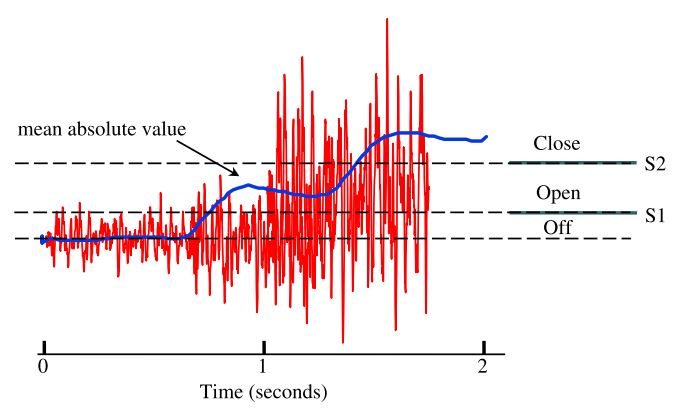
\includegraphics[width=.49\textwidth]{figures/Switch1}}
 	\subfigure[Two channel threshold control.]
 	{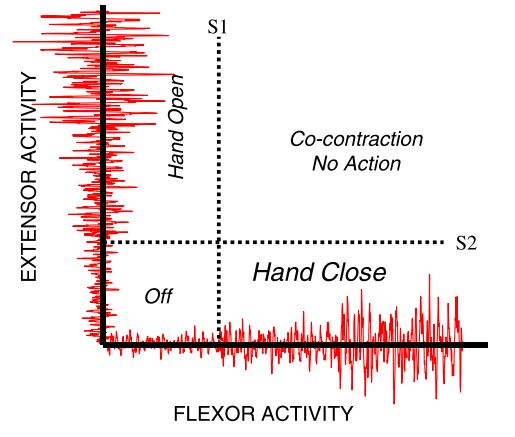
\includegraphics[width=.4\textwidth]{figures/Switch2}}  
 	\caption{Illustration of a direct one channel (a) and two channel (b) threshold control schemes using EMG amplitude to control open/close hand function. S denotes a threshold. Illustration taken from \cite{Parker2006}.}
 	\label{fig:Sw}
 \end{figure}  
   
   
%sequential 
\subsection{Sequential myoelectric control}

To overcome the disadvantages of direct switch-based control in slow and not intuitive control, alternative control strategies relying on algorithms have been derived. Such algorithms could utilize classification-based pattern recognition to predict the intended movement of the user. Often signal from several electrodes are captured. An assumption is that given a consistent movement task is performed the muscles will exhibit a unique activation pattern, and that features extracted from each signal for each movement type can be used to distinguish between different movement types. Hence, complex EMG-signal patterns can be assigned to discrete movement classes, thus also allowing for control of several DoF's.  \cite{Farina2014,Wurth2014}  \\
This approach is more intuitive as it does not demand the need for switching between DoF's, and lowering the amount of effort the user has to put in completing a task. A disadvantage of sequential control is lack of simultaneously controlling multiple DoF's at once allowing for a faster and more natural task execution. \cite{Farina2014}  

%Simultaneous
\subsection{Simultaneous myoelectric control}

Incorporating intuitiveness and naturalness in prosthetic control can be achieved through simultaneous control, where more than one DoF is controlled at a time. Pattern recognition methods predicting more than one movement type have been proposed, but naturalness through proportional actuation speed cannot be achieved independently for each DoF. Instead regression-based methods have been introduced. Compared to classification, which will output one class, trained regressors will continuously output the estimated value for each movement type. Choosing the two movement, which fit the regressors the best will provide simultaneous and proportional control. \cite{Hahne2014} 


\section{Data Processing}
In order to use the acquired data most optimally in the myoelectric prosthetic control scheme the data must be processed. In this processing, undesired frequencies are filtered out and features that represents the data are extracted from segments of the data in order to obtain more information about the movement than what is only contained in the raw EMG signal. This data processing will be covered in the following sections. 

\subsection{Filtering}
To remove unwanted frequencies from the EMG signal, it should be filtered. According to the Nyquist Theorem, the rate the signal is sampled with must be at least twice the highest frequency contained in the signal to archive a non-aliased digital recording. However, as mentioned in \secref{sec:MYO}, the MYB samples with a rate lower than the highest frequency in the EMG spectrum, without having any analogue bandpass filter implemented. The rationale behind incorporating a digital anti-aliasing filter is therefore defeated. Implementing a digital high-pass filter with a corner frequency at 10 Hz to remove low frequency artefacts would, however, be desirable. \cite{Cram2012} 

\subsection{Feature Extraction}
Instead of only utilizing the raw EMG signal in a control scheme, features are extracted to exploit more representations of the EMG signal that optimally results in robust control. Various independent features can be extracted from the signal either from the time domain, frequency domain or the time-frequency domain. Most commonly features from the frequency and time domain are used. When extracting frequency domain features it is required for the EMG signal to transformed into the frequency domain. This takes more computation time compared to extracting features directly from the time domain. For this reason features in the time domain are usually favoured. \cite{Phiny2012} Especially used are the Hudgins features: Mean Absolute Value (MAV), Zero Crossings (ZC), Slope Sign Changes (SSC) and Waveform Length (WL) \cite{Hudgins1993}. However, both ZC and SSC represent the frequency content of the signal, which most likely has been distorted by the low sample rate. When using the MYB for EMG acquisition an alternative set of features has been suggested by Donovan et al. to extract from the data \cite{Donovan2017}. These features are so called space domain feature, since they exploit the relationship between the output from the electrode channels. When evaluating data acquired from the MYB the space domain features increased classification accuracy by 5 \% in a LDA-based control scheme compared to using the Hudgins features \cite{Donovan2017}. A final consideration to make when choosing features is to avoid redundancy as they then would not provide additional information about the signal. 

\subsection{Segmentation}
The extraction of features are done in discretely segmented windows of data, instead of calculating the features from instantaneous values. In online control, the length of windows is a compromise between classification accuracy and delay in prosthetic control. Often an window overlap is implemented. This is a technique applied to ensure short delays, while still enabling a high classification accuracy. When applying an overlap values from the previous window is reused in the current window. The amount of overlap chosen is significant for the performance of the control scheme.  Generally, it is recommended to have window lengths of 150-250 ms and use a 50 \percent overlap. Choosing a large overlap will result in short delays, but worse classification accuracy and vice versa. When using the MYB it is important to take the low sample rate into consideration, as a window will contain less data compared to if the sampling was appropriate to the EMG frequency properties. \cite{Menon2017} Short windows will therefore likely result in worse classification accuracy compared to appropriately sampled data segmented in identical window length.
% but other studies using the MYB for data acquisition have used window lengths of 260 ms with a sliding window overlap of 235 ms \cite{Cote-Allard2017} 

\section{Classification}
For the myoelectric prosthesis to know which movement to perform, it needs to know how to differentiate between the movements it will be trained to perform. For this purpose classification is a commonly applied model. The classification model, or classifier, is given known data consisting of features extracted from the raw EMG signals, which were recorded while the user was performing different movements. If each of the known feature data sets related to each movement is known they can be labelled appropriately, and the classifier will then know which data represents which movement. Each label is known as a class and the process of labelling the data is called supervised learning. The known data is also called training data, hence this process is called training the classifier. If the classifier is trained properly, it is able to categorize unknown data accurately into the correct class. This is what happens online in each segmented data window when using a pattern recognition-based myoelectric prosthesis. The classifier is, however, only able to categorize unknown data into one of the trained classes. \\
A frequently used supervised classifier for myoelectric prosthetic control is the LDA classifier. An advantage of using LDA is that it enables robust control, while having a low computational cost. LDA will be used in this project to determine motor function and an overview of the theory behind LDA will be given in the following section.

\subsection{Linear Discriminant Analysis} 
LDA determines decision boundaries between the desired number of classes, where the distance between the decision boundary and the centroid of the class feature values is maximized. Such a decision boundary is defined as a linear combination of the feature values and a weight $w$:

\begin{equation} \label{eq:LDAcommon}
	g_{j}(x) = weight_{j}x + bias_{j}
\end{equation}

where $weight_{j}$ decides the orientation of the decision boundary of class $j$, and $bias_{j}$ is a bias that decides the position of the decision boundary of class $j$ in relation to origo. \\
The decision rule of a LDA classifier is based on which class that has the highest probability of having produced the input feature values; also called the posterior probability. Given this decision rule, LDA can be derived from the Bayes theorem, which expresses the posterior probability as:

\begin{equation}
	P(\omega_{j}|x) = P(x|\omega_{j})P(\omega_{j})
\end{equation}

where $P(x|\omega_{j})$ is the class conditional probability, the probability that a feature value from class $j$ appears, and $P(\omega_{j})$ is the prior probability, the probability that class $j$ appears. This can be written as the function:

\begin{equation}
	g_{j}(x) = P(x|\omega_{j})P(\omega_{j})
\end{equation}

\\
An constraint in LDA is that each class is Gaussian distributed and all classes share the same covariance matrix. The class conditional probability can therefore be written as the multivariate normal distribution, in which the class conditional covariance matrix can be written as the common covariance matrix. This leaves the following function:

\begin{equation}\label{eq:LDAadvance}
	g_{j}(x) = \mu_{j}\Sigma^{-1}x'-\frac{1}{2}\mu_{j}\Sigma^{-1}\mu'_{j}-ln(P(\omega_{j}))
\end{equation}

where $\mu_{j}$ and $\Sigma^{-1}$ are the mean vector for class $j$ and the common covariance matrix, respectively. The function in \eqref{eq:LDAadvance} can be written in the common linear discriminant classifier form as in \eqref{eq:LDAcommon}. \cite{Scheme2013}\\
Thus, a posterior probability is calculated for each class based on the decision boundaries, and according to the decision rule, the class with the highest probability of having produced the input feature values will be chosen as the determined motor function. However, LDA only determines the movement class, but does not map the motion the actuator must perform. For this purpose am additional control scheme must be applied to activate the determined motor function in a proportional matter. \cite{Fougner2012}

%fitcdiscr(classInput,moveLabel,'DiscrimType','pseudolinear', 'ScoreTransform','none','HyperparameterOptimizationOptions','bayesopt')
%
%pseudolinear: all classes have the same covariance matrix. The matrix is inverted by the used the pseudo inverse
%
%none: the confidence scores are not transformed
%
%bayesopt: uses bayes optimization to yield minimum loss in cross validation
\section{Proportional Control}
After the motor function has been determined, a mapping of the control output needs to be performed. The advantage of providing a continuous output to the actuator proportional to the contraction intensity compared to a one-speed controller is that the user has the possibility of grasping objects quickly, while still being able to perform more slow and dexterous tasks. Additionally, proportional control resembles the human neuromotor system, which makes it more intuitive. \cite{Fougner2012} 

A widely used proportional control scheme is linear regression \cite{Fougner2012}. Here, a dependent output value can be calculated based on a function of an independent input value. In the case of using several electrode channels as when using the MYB, the output needs to be computed based on several independent values. For this purpose multiple linear regression would be appropriate:

\begin{equation}
	\hat{Y} = \alpha+\beta_{1}X_{1}+\beta_{2}X_{2}+\cdots+\beta_{i}X_{i}+\epsilon_{i}
\end{equation}

where $\hat{Y}$ is the control output and $X_{i}$ is the independent input values, where the index $i$ will correspond to the number of electrode channels in the MYB. $\alpha$ and $\beta$ are the estimated value of $\hat{Y}$ at $X$ = 0 and estimated regression coefficients, respectively. The absolute values of the recorded EMG signals can be used directly as the independents input value in such a proportional control scheme. \cite{Zar2009} However, a regression model needs to be estimated for each motor function in the control system. Then the appropriate regression model will be selected based on the classification output.  
\section{Performance Evaluation}

Evaluating the performance of a derived control system can be achieved through the completion of various tasks. If available, the system can be interfaced with a myoelectric prosthesis, and based on the completion of tasks mimicking daily life functionality (e.g. grasp and movement of objects), performance can be evaluated \cite{Mastinu2018}. Otherwise, virtual environments have been widely used showing movements of virtual prostheses \cite{Powell2014} or by moving a cursor to targets resembling motor function, where performance can be quantified through measurements based on Fitts' Law \cite{Scheme2013,Wurth2014,Hahne2014}. An obvious measure to observe is the completion rate (CR), which is the ratio of reached targets compared to the total number of targets. This describes the overall ability the user has when using the control system. Path efficiency (PE) can be used to observe how efficiently continuous movement control is achieved by comparing the distance travelled to reach a target and comparing it to the most direct route. To observe how well the user can keep the system at rest and control velocity, stopping distance (SD) and overshoot (OS) can be measured. The former measures the distance travelled at times where no movement is intended, and the latter tracks the number of times the user reaches a shown target, but leaves before completion. \cite{Scheme2013}


\chapter{Study Objective}


In summary, there is still a need for myoelectric prosthetic devices to fully close the neural loop by providing amputees with proprioceptive feedback to lower the need for visual attention. As presented in \secref{SoA} most studies have focused on providing exteroceptive feedback while only very few studies have investigated how proprioceptive information could be conveyed to aid prosthetic control in cases where visual attention is less wanted. Using the modality of electrotactile stimulation as a mean of transferring information of the prosthetic state offers multiple stimulation parameters which can be modulated through several channels enabling possibilities for intuitive and meaningful sensory feedback. However, even though several opportunities present themselves in modulating the stimulation amplitude, frequency and active channels, it would be of great interest to investigate which would lead the sensory feedback to be perceived most intuitively. As stated in \secref{Maxxx} the frequency cannot be controlled individually for each pad in the electrode, thus a feedback scheme modulating frequency will no be investigated in this study. \\ Investigating whether spatially coded or amplitude coded information assists the most when neglecting visual attention will provide insight into which parameters future configurations should encapsulates. This leaves the following study objective: 

\begin{center}
	\textit{Test and evaluate two novel stimulation schemes, one based on modulating amplitude and one based on spatial localization of activation, for conveying sensory feedback of the prosthesis state in a closed loop prosthetic control system.}  
\end{center} 


\chapter{Methods}


Extending the knowledge acquired involving myoelectric prosthetic control, feedback stimulation and the desire among prosthetic users for prostheses to incorporate proprioceptive feedback, the following section will document the implementation of the two feedback configurations, as well as the rest of the developed closed loop system. The methods chapter will present the following sections documenting the implementation of: study design, data acquisition, data processing, control system and validation of control, spatial configuration, amplitude configuration, configuration training, performance test and statistical methods.      
\section{Study Design}

In order to investigate whether amplitude or spatially-based electrotactile feedback aids prosthetic control the most when removing the visual dependency, an experiment was set up. A feedback coding scheme based on spatial activation and a feedback scheme based on amplitude modulation was developed and will be presented in \secref{sec:feed}. \\
14 able-bodied subjects (13 right-handed, 12 males) were recruited, where the order of which feedback scheme the subjects would be trained/tested in was randomized. However, an equal number of subjects was assigned to each order. An overview of the subject population and demographics can be seen in \tabref{tab:demo}. 

\begin{table}[H]
	\caption{Overview of subject population and demographics.}\label{tab:demo}
	\begin{tabular}{llll} \hline
		& \textbf{Age, mean(std)} & \multicolumn{2}{c}{\textbf{Gender(n)}} \\ \cline{3-4}
		&                & Female          & Male           \\ \hline
		\begin{tabular}[c]{@{}l@{}}\textbf{Total}\\ (n = 12)\end{tabular}   & \multicolumn{1}{c}{26.1(2.4)}    & 2       & 14      \\
		\begin{tabular}[c]{@{}l@{}}\textbf{Order 1}\\ (n = 7)\end{tabular} & \multicolumn{1}{c}{25.7(2.3)}    & 1       & 6      \\
		\begin{tabular}[c]{@{}l@{}}\textbf{Order 2}\\ (n = 7)\end{tabular}    & \multicolumn{1}{c}{26.4(2.6)}    & 1       & 6      \\ \hline
	\end{tabular}
\end{table}

\vspace{-0.4cm}
Prior to enrollment, the subjects were assessed to meet the inclusion criteria stated in the experimental protocol, which can be found in \secref{Ex_protocol}. The subjects were handed a short experiment description prior to the experiment session (see section \ref{SED}), which gave an introduction to the background of the study and the different task the subjects would have to go through. Upon enrollment, the subjects were asked to sign an informed consent form, which stated that the subjects had received adequate information about the experiment and that they were always able to withdraw from the experiment. The experiment was ethically approved by the ethic committee of Region Nordjylland, Denmark (Approval number N-20150075).\\
The experiment was designed such that each subject was trained and tested in using both feedback schemes along with control during a single session experiment. A graphical illustration of the main stages that the subject went through can be seen in \figref{fig:std}. For all subjects data used to build the prosthetic motor control system was acquired first. Secondly, the subjects were given time to familiarize with the control system and subsequently, the achieved control was evaluated through a target reaching test. Next, sensory threshold levels used for feedback were determined for the subject. Subjects assigned to order 1 went through four steps of training and testing using the spatial scheme followed by the same four steps using the amplitude scheme. Subjects assigned to order 2 went through the schemes in opposite order. The next sections will further document the implementation and execution of the experiment.     

\begin{figure}[H]                 
	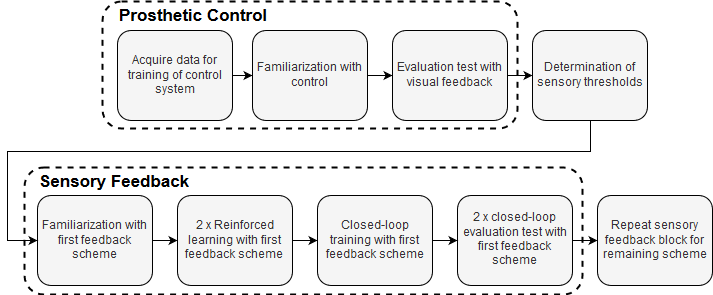
\includegraphics[width=.95\textwidth]{figures/std_paper}
	\caption{Pipeline showing the stages of the experiment. The stages in the first block focused on developing a prosthetic control system, and evaluating the
		subjects’ ability to control the prosthesis. Then electrotactile sensory thresholds were determined. The second block focused on training the understanding of
		the feedback schemes and evaluating their use in combination with prosthetic control. The sensory feedback block was repeated for the remaining feedback
		scheme.}
	\label{fig:std} 
\end{figure}

\section{The Virtual Closed-Loop Prosthesis} \label{sec:vp}

In order to test the usability of the two sensory feedback configurations in a closed-loop control system, a prosthesis which accommodates this was simulated. As no commercial or research prostheses were available in this project, a virtual system resembling prosthetic control was made. Using a virtual prosthesis also had the benefit of providing no sounds that might indicate the prosthesis state. \\
The aim was to develop a system which could provide control and feedback of two degrees of freedom. For this purpose, it was chosen to incorporate the rotational degree of freedom in wrist supination and pronation and a grasp degree of freedom in open and closed hand. In \figref{fig:meth:gridmap} is a depiction of a grid and a cursor dot symbolizing the different possible prosthetic states and the current prosthetic state, respectively. Performing supination would make the cursor move to the right into one of two possible states, while performing pronation would make the cursor move left into one of two states. Performing the closed hand movement would make the cursor move downwards into one of four possible states and performing open hand would make the cursor move upwards. In total, the prosthesis could achieve a total of 25 different states, which represented single DoF movements or combinations of two DoFs. However, as the control was sequential it was only possible to move the cursor in a single DoF at a time. In each of the squares, a unique electrotactile feedback was provided in each of the two feedback configurations, which will be further explained in the later \secref{sec:feed}, thus ascribing four states for each DoF.      
     

\begin{figure}[H]                 
	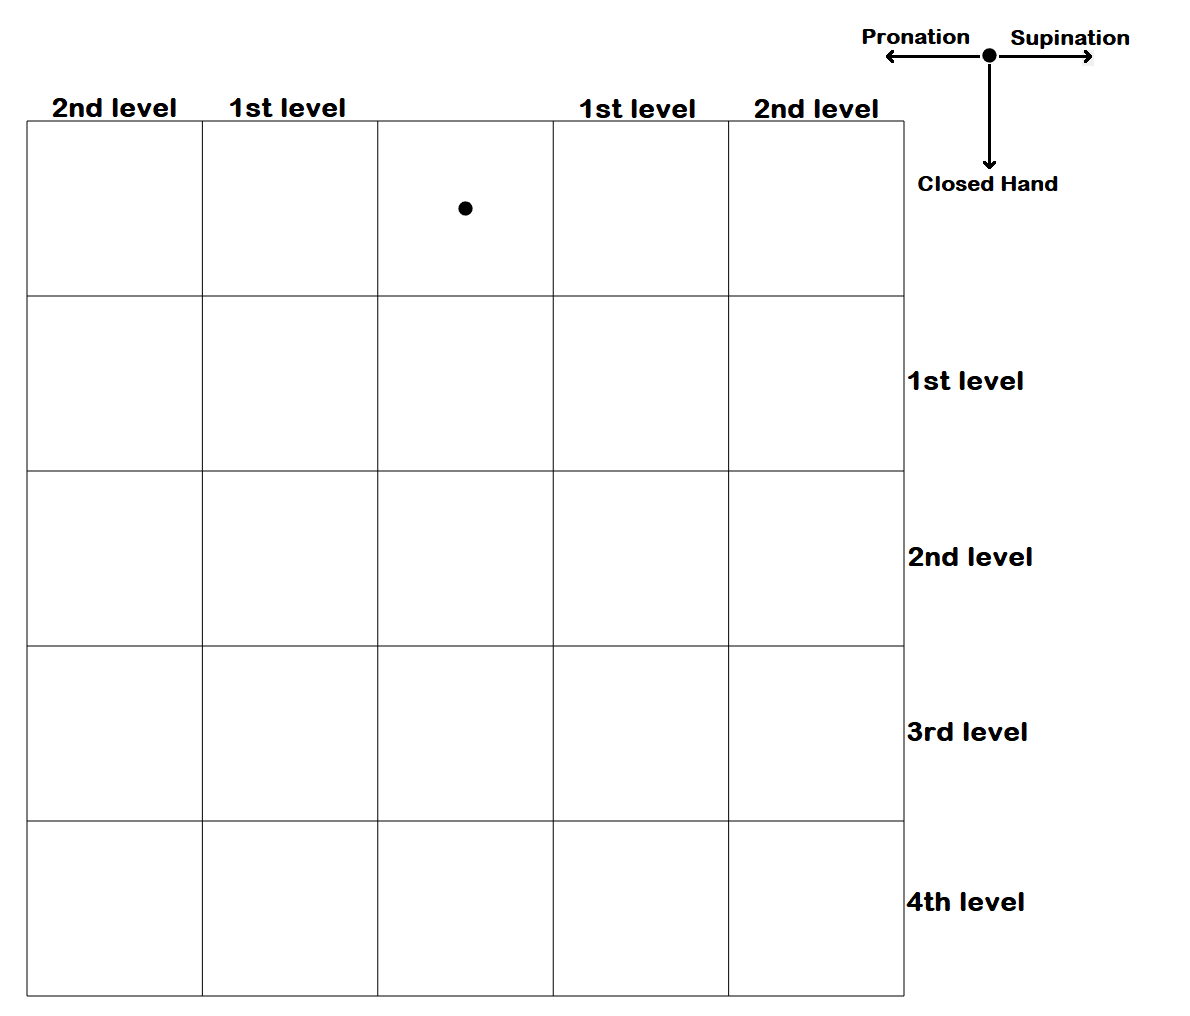
\includegraphics[width=0.9\textwidth]{figures/gridmap2}  
	\caption{Image of the grid map and cursor used in the experiment. Performing supination moves the cursor to the right, pronation moves it to the left and closing the hand moves it down. Opening the hand moves the cursor up, and was used as a correction movement if needed.}
	\label{fig:meth:gridmap} 
\end{figure}
%hand movements used 

%The Grid 

\section{Acquiring Training Data}

As presented in \secref{patter}, for the classification scheme to differentiate between movements, it has to be trained with EMG data from each movement. Training data was acquired using the MYB placed on the forearm and recorded the movements of pronation, supination, open hand, closed hand and rest. The subsequent section will document how the data used for training the classifier was acquired. \\
First, a baseline recording was made, where the subject was instructed in keeping the hand perfectly still. The baseline consisted of a 15 second recording and was subtracted from each of the other recordings to reduce baseline noise. If the signal was below the baseline amplitude it was set to zero. \\
During a muscle contraction two main states can be recognized; a transient state, described by inconsistent myoelectric activity as the muscle length is changed and steady state, where a constant firing rate is reached. \cite{Mobarak2014} Classification is often based solely on steady state data and even though incorporating transient state in the training data has been found to decrease classifier accuracy \cite{Mobarak2014}, including transient state might make for a more robust classifier as the delay until steady state is reached is eliminated \cite{Boschmann2013,Mobarak2014a}. \\
%

\begin{figure}[H]                 
	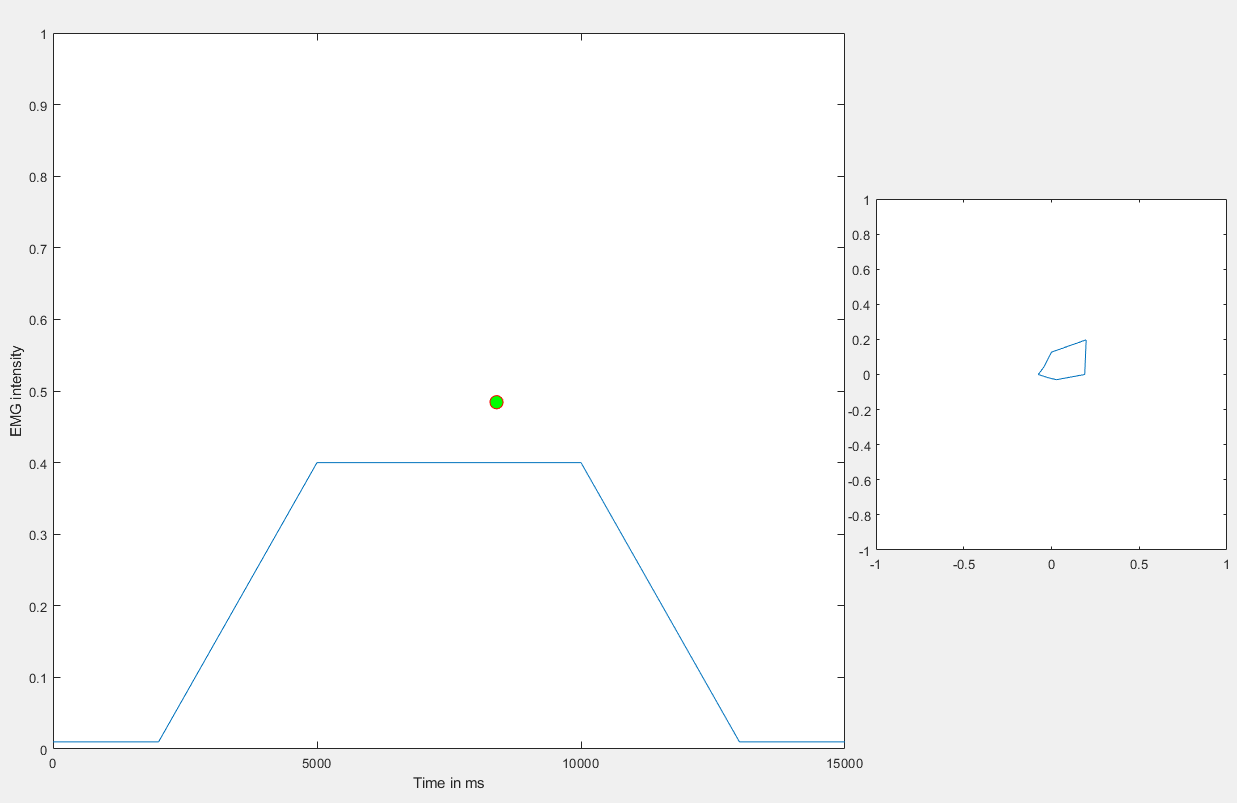
\includegraphics[width=.8\textwidth]{figures/dataacqGUI}  
	\caption{The trapezoidal plot (left) and contraction validation plot (right) used during acquisition of the training data. The line in the trapezoidal plot represented the contraction amplitude requested and the green cursor represented the current elicited contraction intensity. }
	\label{fig:GUI} 
\end{figure}
\vspace{-1em}

To feed the classifier with training data representing muscle contractions with varying force, different fractions of maximum subject contraction force were recorded. The process of obtaining training data for each movement the same four step process of a Maximum Voluntary Contraction (MVC) recording and a 40 $\percent$, 50 $\percent$ and 70 $\percent$ fraction of MVC recording.
The MVC was recorded for 15 seconds where the subject was instructed to elicit the contraction with a maximum contraction force which could be held steady, without fatigue, over the course of the 15 seconds. This resulted in an MVC for each channel in the MYB. The absolute of the EMG signal for each channel was computed and a mean across all channels was calculated. The mean was used as reference when recording the subsequent training data. \\
Acquisition of the 40 $\percent$, 50 $\percent$ and 70 $\percent$ fraction of MVC, were done using a developed graphical user interface (GUI), which can be seen on \figref{fig:GUI}. The image shows the trapezoidal figure, which line the subjects were instructed to follow using the green cursor, which was a representation of the mean intensity across all channels of the elicited muscle contraction. The cursor would automatically move forward along the x-axis in relation to time. The height of the trapezoid represented either the 40 $\percent$, 50 $\percent$ or 70 $\percent$ fractions of the MVC. Data were recorded during 2.5 seconds rest periods in the beginning and end, a 2.5 incline transition, 5 second steady state and 2.5 second decline transition, summiting to a total time of 15 seconds. However, only data recorded during the steady state and last and first second of the incline and decline transition phase, respectively, were extracted and to be used for training the classifier. \\
The additional plot seen on the right in \figref{fig:GUI}, plotted the amplitude of each of the eight channels in the MYB and were used by the investigators to assess whether the performed movements were done correctly. If sudden shifts in the amplitude or the channels activated were present, this would indicate that the subject did not perform a pure contraction and the recording would have to be redone.   
   
   

\section{Data Processing}
The following sections will cover which filtering, segmentation and feature extraction solutions that were decided to implement, based on the background information presented in \secref{sec:BG:dataProcessing}. 

\subsection{Filtering}
Due to the EMG bandwidth being 10-500 Hz and taking the MYB specifications into consideration the only interest was to remove low-frequency artefact noise. Hence, a $2^{nd}$ order Butterworth high-pass filter with a cut-off at 10 Hz was implemented. The order of the filter was chosen, as fast update time was highly desired in the online prosthetic control, and a higher order might have slowed the update due to a longer computation time. The choice of implementing a Butterworth filter was due to the desire of minimizing phase shift inside the EMG bandwidth, as this could further distort the fidelity of some of the extracted features. 

\subsection{Segmentation}
In online myoelectric prosthetic control, quick update time is important to maintain naturalness in the prosthesis motion, while still ensuring robust classification. A windowing of 200 ms with 50 \% overlap was therefore chosen. This would update the prosthesis position every 100 ms and segment 40 samples per window to feed the classifier. In initial tests, this proved adequate to yield smooth and reliable prosthesis motions, when using the MYB for EMG acquisition. 

\subsection{Feature Extraction}
For this project it was decided to extract the space domain features recommended by Donovan et al. \cite{Donovan2017}, due to the increased classification accuracy obtained compared to using Hudgins features when applying the MYB for data acquisition. The features formulated in \cite{Donovan2017} were MAV, Mean MAV (MMAV), Scaled MAV (SMAV), Correlation Coefficient (CC), Mean Absolute Difference Normalized (MADN), MAD Raw (MADR) and Scaled MADR (SMADR). Additionally, it was decided to extract the Hudgins feature, WL, to exploit frequency related information of the signal in the classification. All these features will be explained in the following text. 

MAV is a commonly used feature to represent information on muscle contraction intensity and how much force a subject needs to produce to perform a movement at a given intensity. Its changes are linearly proportional with contraction intensity; the more intense the contraction is the higher the feature value will be and vice versa. For one window in the $i^{th}$ channel, MAV is calculated as:

\begin{equation} \label{eq:MAV}
MAV_i=\frac{\sum\limits_{n=1}^{ws}|x_i[n]|}{ws}
\end{equation}

where $x_i[n]$ denotes the $n^{th}$ raw sample from channel $i$ and $ws$ denotes window size or number of samples in one window. \\
Scaling MAV with the mean of MAV across all channels will remove the dependency of specific movement intensity - some movements produce higher mean intensities than others at the same fraction of the pMVC. The average of MAV across all channels is denoted MMAV and is calculated as: 

\begin{equation} \label{eq:MMAV}
MMAV=\frac{\sum\limits_{i=1}^{8}MAV_i}{8}
\end{equation}

MAV scaled by MMAV is denoted SMAV and is calculated as follows for each window in the $i^{th}$ channel:

\begin{equation} \label{eq:SMAV}
SMAV_i=\frac{MAV_i}{MMAV}
\end{equation}

Each EMG channel in the MYB records a mixture of sources. Some individual sources can affect multiple channels, which will increase the correlation between channels, while other more local sources might only affect a single channel, which decreases the correlation. To represent the correlation between channel $i$ and the neighbouring channel $i+1$, Donovan et al. proposed the calculation of a correlation coefficient (CC), which is expressed as: 

\begin{equation} \label{eq:CC}
CC_i=\frac{\sum\limits_{n=1}^{ws}X_i[n]X_{i+1}[n]}{ws}
\end{equation}

where $X_i[n]$ is the $n^{th}$ sample from channel $i$ in one window after the sample has been normalized. The normalization is done by subtracting the mean of raw samples from each sample followed by dividing the resulting values with their standard deviation.  

In an effort to further represent the relationship between channels, the mean of the absolute value of the difference between normalized channel values was calculated. This is referred to as mean absolute difference normalized (MADN), and is expressed as:

\begin{equation} \label{eq:MADN}
MADN_i=\frac{\sum\limits_{n=1}^{ws}|X_i[n]-X_{i+1}[n]|}{ws}
\end{equation}

To decrease the computational denseness of first calculating the normalized values as done with CC and MADN, MAD was calculated using just the raw samples. This is referred to as MADR and is expressed as:

\begin{equation} \label{eq:MADR}
MADR_i=\frac{\sum\limits_{n=1}^{ws}|x_i[n]-x_{i+1}[n]|}{ws}
\end{equation}

Similar to MAV, MAD is affected by movement intensity and is therefore scaled by MMAV, which results in the final space domain feature SMADR: 

\begin{equation} \label{eq:SMADR}
SMADR_i=\frac{MADR_i}{MMAV}
\end{equation}

Finally, to increase the amount information the classifier based its decisions upon, the Hudgins feature WL was included. WL represents both amplitude and frequency content of the signal by measuring the summed absolute difference between neighbouring samples in the signal in channel $i$ in one window: 

\begin{equation} \label{eq:WL}
WL_i=\sum\limits_{n=1}^{ws-1}|x_{i}[n+1]-x_i[n]|
\end{equation}

To avoid redundancy in signal representation only SMAV, CC, MADN SMADR and WL were used to train the classifier and for online control. 


\section{The Prosthetic Control System}

Having extracted features from the three EMG datasets of one movement for each of the four movements, the control system could be build in order to achieve online recognition of movements. The implementation of the control system was divided into two parts. To achieve recognition of performed movement a classifier was trained, however, this only produces a recognition of a movement and does not reflect the intensity of which the movement is being performed with. Therefore, following the recognition of the performed movements a linear regression model was implemented to achieve proportional control. 

\subsection{Movement Classification}

Online classification of movements was accomplished by implementing a LDA classifier. As presented in \secref{patter} the classifier needed to be trained using data from each movement. Hence, the five features extracted for each of the 40 $\percent$, 50 $\percent$ and 70 $\percent$ fraction of the pMVC for one movement were assembled into one labeled matrix. The same was done for the three remaining movements. A fifth class was labeled rest and its matrix only contained the features from a single rest acquisition. These matrices were made for the data acquired from each of the eight channels in the MYB. All matrices were assembled into one training matrix with labels for each movement. Using the \textit{fitcdicsr}-function in MATLAB a LDA classifier was trained by feeding it the training matrix. Hereby, the classifier was trained in separating 5 classes using linear decision boundaries. During online use, the \textit{predict}-function was used to evaluate features from new input data in the classifier and decide which movement there was being performed.    


\subsection{Proportional control}  
When a movement was decided upon by the classifier, the proportional control provided the control system with an actual output to move the virtual prosthesis. For this purpose a multiple linear regression model was created for each of the four movements, through the MATLAB function \textit{fitlm}. The models were fitted with the MAV features extracted from the fraction of pMVC data as well as the mean of the pMVC data. The data was scaled such that the pMVC data was set to 1 and the remaining data was scaled in relation to that. In the online control, the output of the decided regression models was written such that it would move in the direction described in \secref{sec:vp}. The output from the regression models was limited to a maximum of 1, meaning that maximum level of activation detecting was the pMVC level. This was equivalent to moving the cursor 1 cm on the computer screen per segment (100 ms). Thus, the cursor had a maximum speed of 1 cm per 100 ms. As the grid system was quadratic with 20 cm in length, each DoF had a full actuation speed of 2 seconds at maximum activation. Another threshold implemented was a minimum activation of at least 15 $\percent$ for a movement to count, otherwise no output would be provided. This idea behind this implementation was to provide a more stable resting state in addition to the classifier. 


\section{Online Control Training and Test} \label{sec:meth:contraintest}

After the acquisition of data training data and the training of the classifier, two stages where the subject could familiarize themselves with the control and test how well they were able to use the control system, were implemented. It was highly critical that the subject was able to achieve sufficient control abilities such that it would not be due to poor control that a subject was not able to perform well when combined with sensory feedback in the final evaluation tests. However, as the classifier only had five classes, representing five separable movements to distinguish between, a robust online control was achieved in an evaluation test during pilot tests after short training trials. Therefore, the need for subject training could be kept to a minimum.  

\subsection{Familiarization with Control} \label{sec:meth:contrain}

At first, the subject was presented with an image of the grid, which can be seen in \figref{fig:meth:gridmap}, in \secref{sec:vp}. The subject was able to control a cursor and navigate around inside the grid by performing supination to go right, pronation to go left, open and closed hand to go up and down, and rest to stand still. The familiarization was separated into two stages. In the first stage, the user had three minutes to get acquainted the functionality of the control moving the cursor shown in \figref{fig:C1} (a). The cursor acted as a direct output of the control. During the three minute familiarization, the subject was instructed in training unflawed performance of each movement and the transition from a movement to rest. In the second stage, the visual feedback in the form of the cursor was made more discrete. This was done by making the cursor invisible and instead highlighting the outlines of the target that contained the cursor. This discretized cursor representation was included to make the visual feedback identical in resolution to the sensory feedback. The discrete visual feedback can be seen in \figref{fig:C1} (b). Again the subject had three minutes to familiarize with the control. 

\begin{figure}[H]
	\subfigure[Illustration of the cursor used during the first familiarization stage.]
	{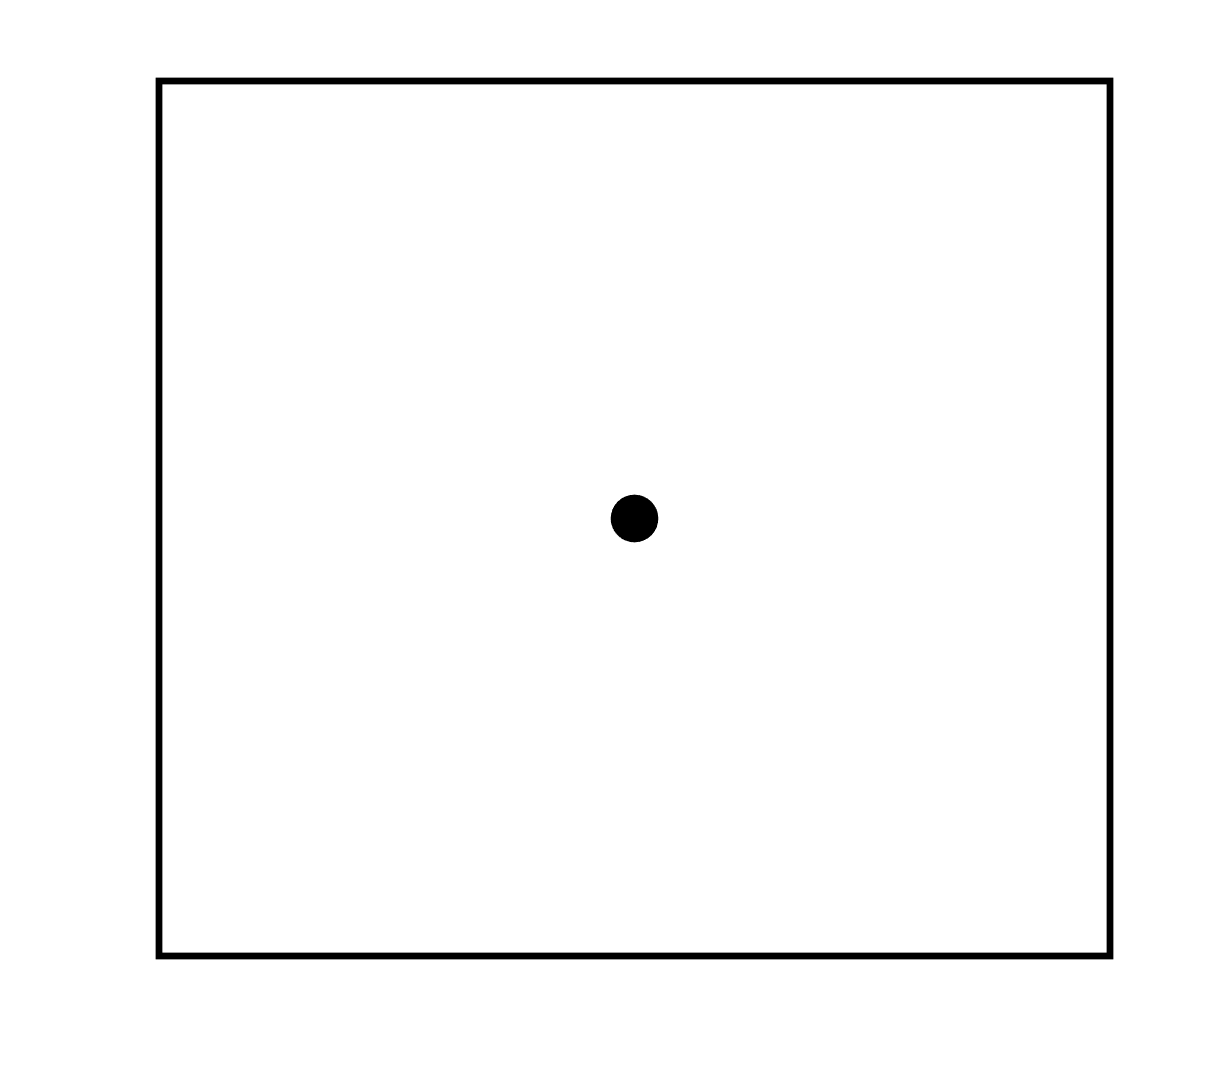
\includegraphics[width=0.34\textwidth]{figures/cursor}}
	\hspace{0.9cm}
	\subfigure[Illustration of the cursor used during the second familiarization stage. ]
	{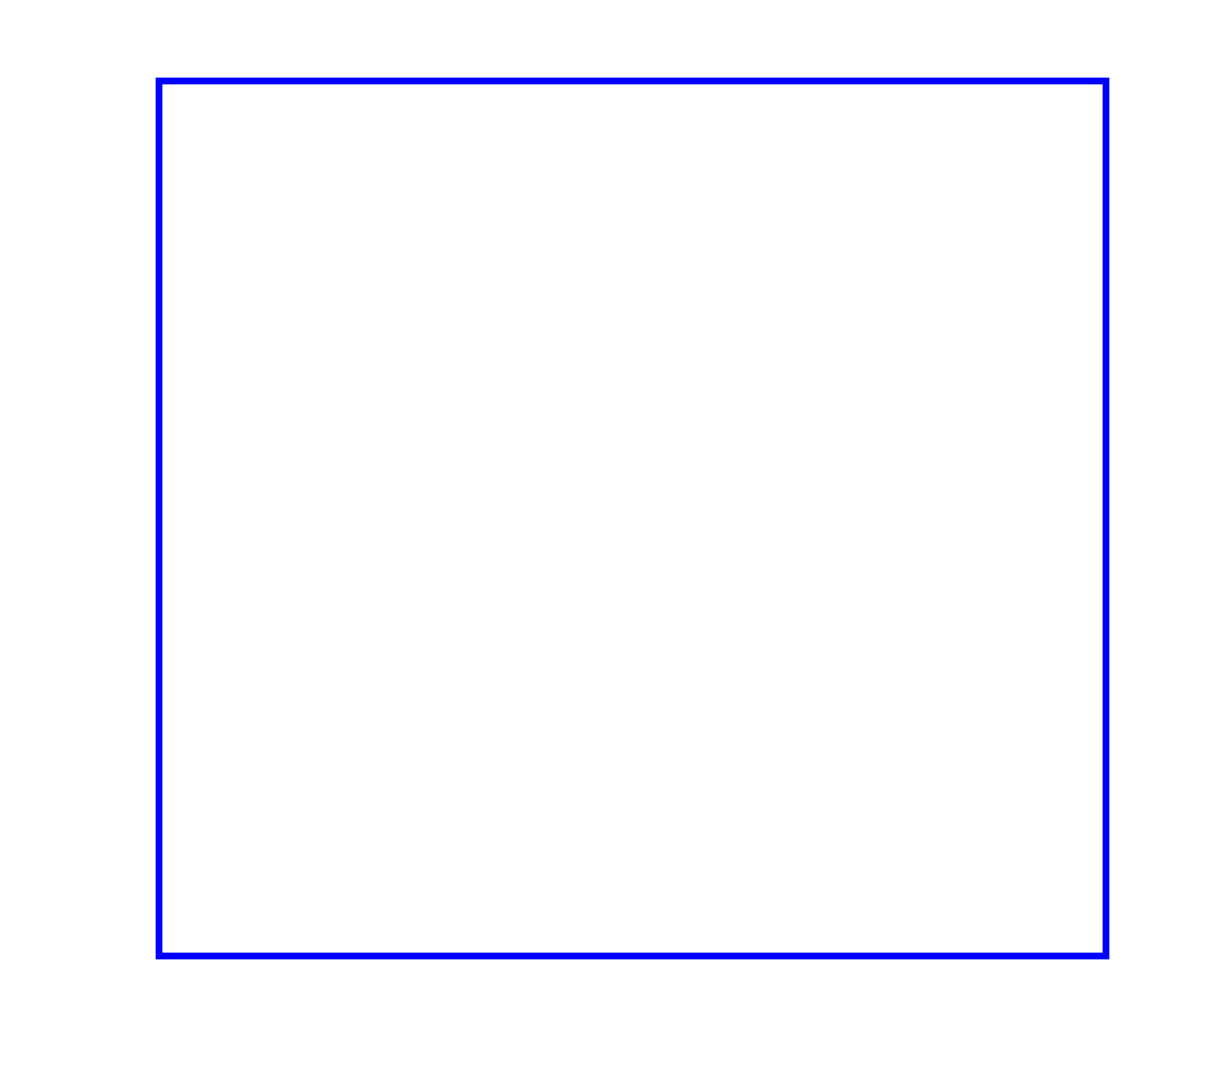
\includegraphics[width=0.34\textwidth]{figures/blue}}
	\caption{Illustration of the cursor used in the two stage familiarization with control.  Using this cursor in (a) the subject was informed the exact location of cursor in a square. Using this cursor in (b) the subject was provided with the information of which square the cursor was in, but not the exact location of the cursor inside the square. }
	\label{fig:C1}
\end{figure}

\subsection{Evaluation Test} \label{sec:meth:contest}

After completion of the two stages of familiarization, a target reaching test was carried out. In this project, performance evaluation will be carried out in a virtual environment through a Fitts' Law based target reaching test. In this test, a square was highlighted with red and the subject would have to move the discretized cursor to the desired target and dwell inside it for 1.5 seconds in order for it to be deemed reached. The subject had 30 seconds to reach a target. The test was designed such that each of the 24 squares in the grid was to be reached. When a target was either reached or the time to reach the target ran out, the cursor would be reset to the neutral position (first row, third column in \figref{fig:meth:gridmap}). \\
The target reaching test was made such that a measure of how well the subjects was able to use the control system could be obtained. Hereby it also acted as a reference for the later comparisons with control in combination with the two feedback schemes. Furthermore, if the investigators deemed the achieved subject control insufficient, the investigators could choose to exclude the subject. This was assessed empirically from observing the subject performance during the control training and quantitatively by evaluating the results of the target reaching test. From the target reaching test, performance measures of completion rate, time to reach a target and length travelled to reach a target were extracted for performance evaluation.



\section{Determination of Stimulation Levels}

Having completed the prosthetic control part of the experiment, the next step was to determine the subject's sensory threshold levels, which would be used to convey feedback information.

In order to provide meaningful tactile feedback to the subject, a range of distinguishable sensory threshold levels had to be determined for the subject. As presented in \secref{sec:vp} the virtual prosthesis had a range of one to four states. Hence, four thresholds based on amplitude values were determined to accommodate four levels of feedback in the amplitude scheme. Furthermore, since the sensory sensitivity varies across different locations of the circumference of the arm, the sensory threshold levels had to be determined for each individual pad in the electrode armband. Sensory threshold levels were found by slowly increasing the amplitude while fixating the pulse width and frequency at 500 $\mu$s and 50 Hz, respectively. 

In the first round, the lowest level was determined, which will be referred to as the perception threshold. For each pad, the amplitude was set to start at 0 $\mu $A and then increase in steps of 100 $\mu$A per second. The subject was instructed in reporting when electrical stimulation could be sensed and that the subject was sure the activated pad was the origin of the perceived stimulation. The pad was deactivated and reactivated once more with the determined amplitude value for a second verification. This process was carried out for each pad starting from pad 1 to 16. Subsequently, the subject was presented with the determined amplitude values in each pad, such that the sensation in the current pad was compared to the neighboring pad. This was carried out such that the determined amplitude values could be readjusted to achieve more homogeneous sensation intensities across all pads.  

In the second round, the fourth level thresholds, referred to as tolerance threshold, were determined using the same procedure as in round one. The tolerance threshold was defined as the highest amplitude the subject felt pleasant. The starting amplitude was in this round, however, the perception threshold. The amplitude was set to increase in steps of 200 $\mu$A per second. The amplitude was increased until the subject reported that the threshold was reached, the stimulation was causing functional muscle activation or a maximum of 10000 $\mu$A was reached. Again the amplitude values were readjusted to achieve homogeneous sensation intensities. Throughout the process of determining sensory threshold levels, the subject was facing away from the computer screen to avoid bias from observing the visual increase of amplitude values.  

Intermediate threshold levels 2 \textit{lvl2} and 3 \textit{lvl3} were calculated for the $i^{th}$ pad based on the perception \textit{p} and tolerance \textit{t} threshold levels as: 

\begin{equation}
lvl2_i = p_i + \frac{1}{3} \cdot (t_i - p_i)
\end{equation}

\begin{equation}
lvl3_i = t_i - \frac{1}{3} \cdot (t_i - p_i)
\end{equation}

       
\section{Feedback Configurations} \label{sec:feed}

The fundamental interest of this project was to develop two novel, intuitive and useful feedback schemes to convey perception information through electrical stimulation and evaluate which one would aid control them most. The following section will present the spatial and amplitude feedback schemes.     

\subsection{Spatial Configuration}

The spatial feedback scheme was created with the interest of achieving an intuitive way to convey the feedback by focusing stimulation to localized regions on the skin. An illustration of the spatial feedback scheme can be seen in \figref{fig:spatial}. The intent was to break the down the number electrode pads down into two groups, one upper and one lower. The upper eight pads (5-12) were used to convey information of the rotational DoF using four pads for either side.  The four pads were divided into pairs of two, where the first from the center in e.g. pronation would be activated when the cursor entered the first level in the grid system.\fxnote{some of our thoughts to why we do it this way maybe. Like why pairs of two and not just one with space between} Likewise, would the second level pair activated when the cursor entered the second level. Hence, during a transition from neutral to level one and level one to level two, the subject should feel the stimulation moving either laterally or medially depending on the position of the cursor. Finally, this means that when the virtual prosthesis in a supinated state the stimulation should be felt in the superior lateral region of the arm, while when the virtual prosthesis is in a pronated state stimulation should be felt superior medial region of the arm.   \\
The lower eight pads (1-4 and 13-16) were used to convey information on open/closed hand. The pads were paired in an opposite manner for each of the four levels respectively, e.i. 4 and 13, 3 and 14, 2 and 15 and 1 and 16. As the hand would move to one closed state out of four possible, a certain pad pair would activate. Transiting from neural to fully closed, the subject should feed the stimulation converging on the inferior side of the arm. The virtual prosthesis was able to take states, which was a combination of the two DoFs. In these cases the feedback would be a combination of any upper and lower pair, resulting in the activation of four pads simultaneously. In the spatial feedback scheme, it was chosen to use the second amplitude threshold determined to enhance the subject's perception of the stimuli. 

\begin{figure}[H]                 
	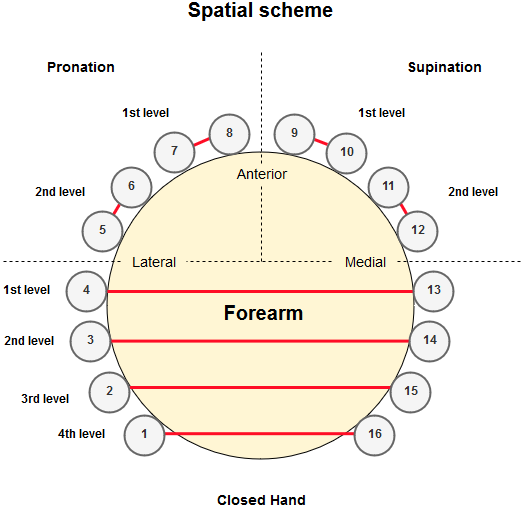
\includegraphics[width=0.55\textwidth]{figures/El_array_spatial}  
	\caption{Illustration of the developed spatial scheme, which is based on different pads being activated depending on the level of the state the cursor is located in. The highest number of possibly activated pads is four at a time.}
	\label{fig:spatial} 
\end{figure}


\subsection{Amplitude Configuration}

Compared to the spatial configuration where the feedback was giving through dynamically changing the pads activated, the amplitude configuration instead conveyed feedback in three greater regions and solely modulated the amplitude of the stimulation. The upper eight pads were again used for the rotational DoF, illustrated in \figref{fig:amplitude}. Pads 5-8 were activated at pronated states using threshold levels 2 and 3 for states 1 and 2, respectively. The same was applicable for supinated states using pads 9-12. \\
For conveying information about open/closed hand pads (1,2,15,16) were used. In these, threshold levels 1-4 were used for states 1-4, respectively. In this scheme, attention to the recognition of stimulation localization should be less. Instead, the subject would have to focus on discriminating between the intensity of stimulation in the regions which are active.          

\begin{figure}[H]                 
	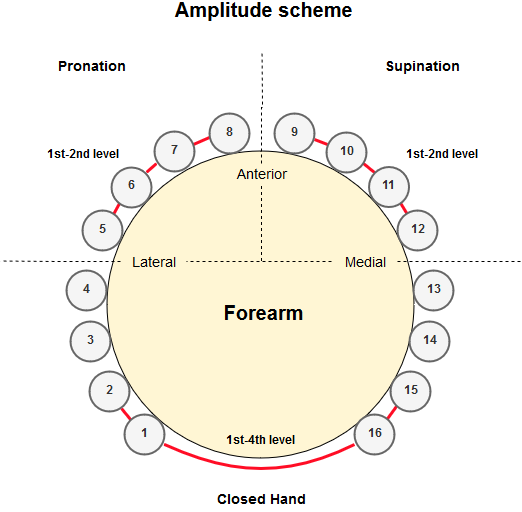
\includegraphics[width=0.55\textwidth]{figures/El_array_amplitude}  
	\caption{Illustration of the developed amplitude scheme. Here, the amplitude of the active pads will increase with the increase of the state. The highest number of possibly activated pads is eight at a time.}
	\label{fig:amplitude} 
\end{figure}








\section{Feedback Training}
After determining the amplitude thresholds, the subject was trained in understanding the sensory feedback. Depending on which group the subject was allocated to, the subject was either trained in understanding the spatial or amplitude scheme first. The structure of the training was, however, the same. The feedback training was divided into two phases: familiarization and reinforced learning. These phases will be presented in the following sections.

\subsection{Familiarization} \label{sec:meth:FBtrainingFam}
In the familiarization phase, the subject was presented with the sensation of 12 different grid squares and 12 grid squares indirectly, while observing which grid location corresponded to which sensation. This was carried out by the investigators by moving the cursor seen in \figref{fig:gridmap_FBfam} with the arrow keys on the keyboard. One press with an arrow key would move the cursor in a different grid square in the direction relative to the arrow key pressed. Pressing return would place the cursor in the staring point (the third grid square in the first row). The order of which grid square the cursor would be moved to can be seen in \figref{fig:gridmap_FBfam}. After reaching a designated square, the cursor would be reset to the starting point. When moving the cursor to a grid square not adjacent to the staring point, the feedback from the transition grid squares would be felt. This transition is transferable to practical proportional prosthetic control/feedback, where the transition from rest to an outer prosthetic position is apparent. When moving the cursor to the grid squares 9, 10, 11 and 12, representing combined DoF positions, the direct route (moving fully in one direction and then the other) was used. In the familiarization phase, the cursor would be moved fully horizontally and then vertically. This enabled stimulations relative to all grid square to be included in the familiarization, without setting all grid squares to be designated targets. This design was chosen due to the single DoF direction being assessed to be most important to get familiar with, and to save time while still exposing the subject to all possible stimulations. Time spend in designated squares was approximately four seconds and time spend in transition squares was approximately two seconds.

\begin{figure}[H]                 
	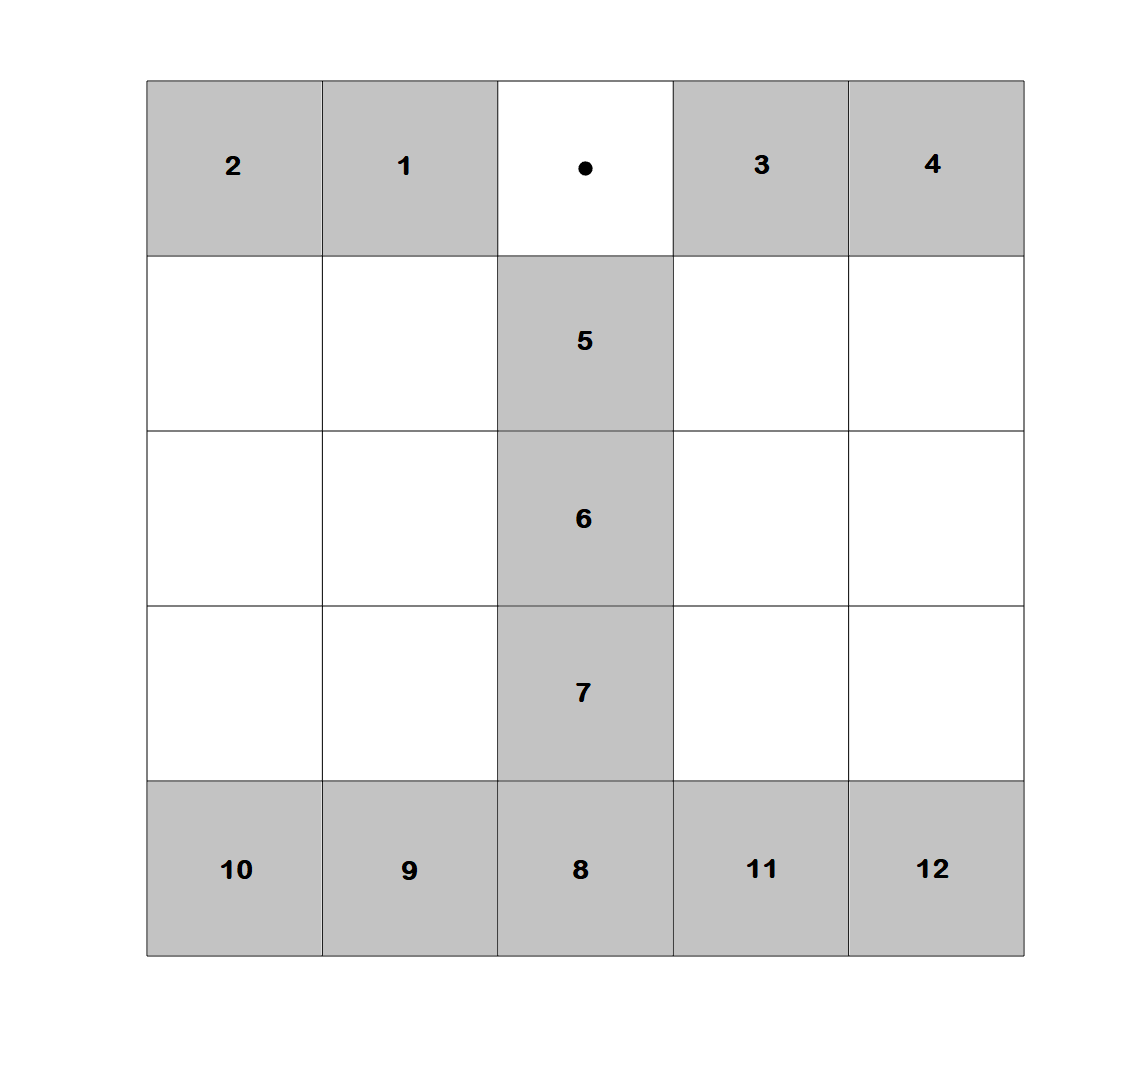
\includegraphics[width=0.55\textwidth]{figures/gridmap_FBfam}  
	\caption{Illustration of the order the cursor would be moved to which grid squares in. The numbered grey squares are designated squares. After reaching a designated square, the cursor would be reset to staring position (the grid square the cursor is located in).}
	\label{fig:gridmap_FBfam} 
\end{figure}

\subsection{Reinforced Learning} \label{sec:meth:FBtrainingRe}
The reinforced learning phase consisted of two blocks, in which all grid squares were designated squares. When a designated square was reached the investigator asked the subject about the location of the cursor. If the subject answered incorrectly, the investigator would reveal the actual location of the cursor. The stimulation related to the designated would be active until the subject answered. Afterwards, the cursor would be reset to the starting point. \\
The difference between the two blocks was the order and path to the designated squares, which was predetermined by the investigators. The blocks were, however, identical for all subjects. The path to a designated square was the direct route. However, which direction that would be moved in first was predetermined by the investigators. Thus, the transition stimulations would be felt by the subject before the designated was reached. This design was implemented to avoid bias in being accustomed to always receiving stimulation related to the same DoF first before the other. Time spend in transition squares was approximately two seconds. 
\section{Combining Control and Sensory Feedback}
After the subject was trained in understanding one of the feedback schemes, the sensory feedback was combined with prosthetic control. Similar to the control step of the study, see \subref{sec:meth:contraintest}, the subject would go through a familiarization phase before undergoing evaluation tests.  These stages will be explained in the following sections. An illustration of the full experiment setup used in this trial can be seen in \figref{fig:meth:setup}.

\subsection{Familiarization}
This stage was similar to the second stage control training, see \secref{sec:meth:contrain}, with the addition of receiving sensory feedback. The subject was instructed in refreshing the prosthetic control, while adapting further to the feedback related to the various prosthesis states as well the transitions felt when changing prosthesis state. These focus point were assessed most beneficial to train in order to perform well in the final evaluation test. The duration of the familiarization phase was three minutes.

\subsection{Final Evaluation Test}
This evaluation test was similar to the evaluation test from the control step, see \secref{sec:meth:contest}, with the addition of receiving sensory feedback. In this test, the prosthesis state would, however, not be visualized. Thus, the subject had to use the sensory feedback to determine the prosthesis state and reach the highlighted targets. The target reaching test was performed two times consecutively. Again the completion rate, time to reach a target and length travelled to reach a target were extracted for performance evaluation.

\begin{figure}[H]                 
	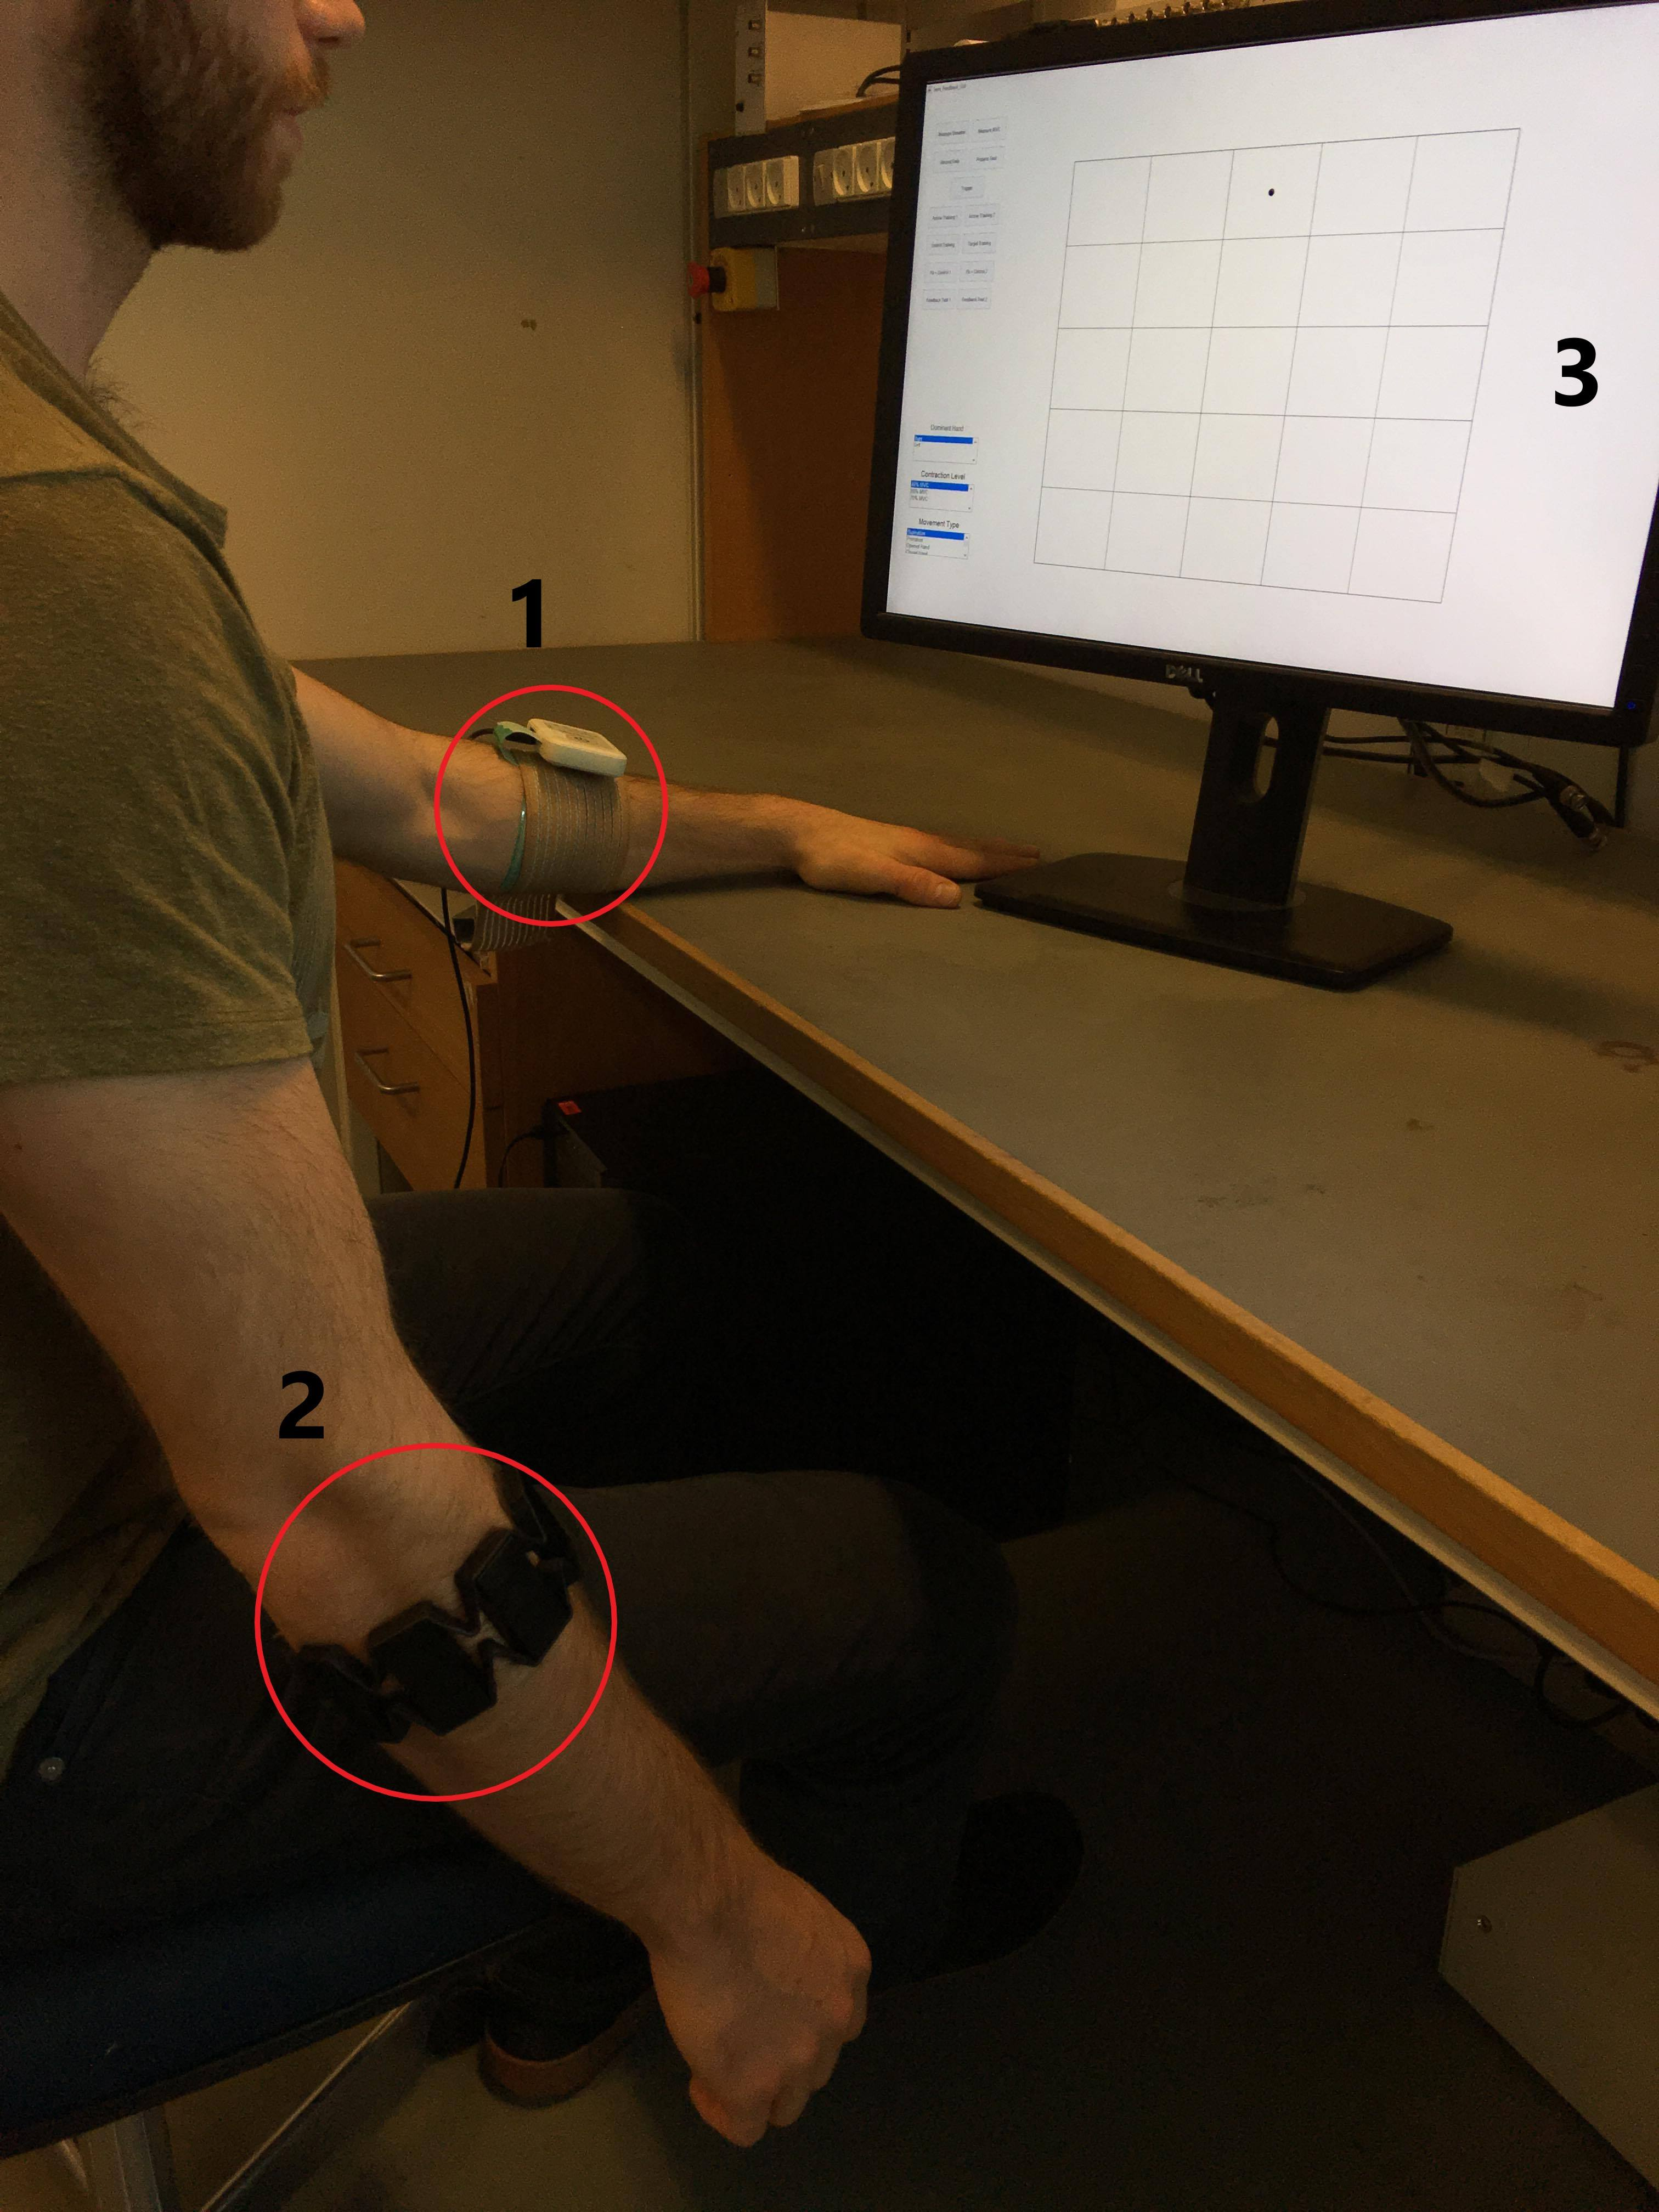
\includegraphics[width=0.8\textwidth]{figures/setupimg}  
	\caption{Image of the experimental setup. 1) is the stimulation device with the stimulation electrode placed under the brown armband, 2) is the electrode armband used to record EMG signals and 3) is the computer screen used to guide the subject and display tasks.} 
	\label{fig:meth:setup} 
\end{figure}

\chapter{Results}


\section{Statistics}
Due to the low sample size, comparisons was made using non-parametric statistics. Wilcoxon signed rank test was applied as comparisons was made on related samples obtained from a two block study design. A significance level of 5 $\percent$ was used.
	
\urlstyle{same}
\printbibliography
\clearpage



\cleardoublepage
% BILAG
\begin{appendices}
\chapter{Appendices}
\section{Experiment Protocol} \label{Ex_protocol}

\textbf{Project Title} \\
Evaluation of electrotactile feedback schemes in combination with myoelectric prosthetic control - closing the loop. 

\textbf{Information on Investigators} \\
The investigators are Biomedical Engineering Master students at Aalborg University. 

\textbf{Background} \\
Losing an upper limb can be hugely debilitating and can result in lowered quality of life due to restrictions in function, appearance and sensation. As a mean to regain the functionality, transradial amputees can receive a functional prosthesis, where the majority are controlled by muscles signals, or myoelectric (EMG) signals. However, still 25\% of myoelectric prosthesis users reject their device, where a major reason for the low satisfaction is due to lack of sensory feedback.
Many advancements have been made in the academic community to improve function accuracy. However, combining function with sensory feedback, thus closing the motor/sensory loop, is still a scarcely investigated area. Therefore, this experiment will combine the control of a prosthesis with sensory feedback delivered via electrotactile stimulation electrodes placed on the forearm. During the experiment the subjects will test two different feedback configurations while controlling a virtual prosthesis, represented as a cursor on a computer screen. The subject can move the cursor in a two-dimensional coordinate system, where the axes represents a degree of freedom (DOF) each (wrist rotation and opened/closed hand).

\textbf{Purpose} \\
The purpose of the experiment is to compare how subjects' perform in an evaluation test when receiving feedback from two different electrotactile stimulation configurations, respectively, in a closed loop virtual prosthesis. This might provide information on which feedback that seems more intuitive to use in practice in a prosthesis.

\textbf{Research Aim} \\
Test and evaluate two novel stimulation schemes, one based on modulating amplitude and one based on spatial localization of activation, for conveying sensory feedback of the prosthesis state in a closed loop prosthetic control system.

\textbf{Experiment Duration} \\
Approximately 2 hours and 30 minutes.

\textbf{Inclusion Criteria} \\
The subject must be:
\vspace{-15pt}
\begin{itemize}
	\item able bodied. % or transradially amputated as the highest degree of upper limb amputation.
	\item at least 18 years of age.
	\item able to understand, read and speak English and/or Danish.
	\item assessed by the investigators to comply with the instructions given during the experiment.
\end{itemize}

\textbf{Exclusion Criteria} \\
The subject must:
\vspace{-15pt}
\begin{itemize}
	\item not have any diseases/conditions that may influence sensory perception.
	\item be willing to receive low amplitude current stimulation. 
	\item be assessed by the investigators to have robust prosthetic control during the experiment. 
	\item be willing to give informed consent. 
\end{itemize}

\textbf{{\Large Experiment Description}} \\
\newline
The main aim of the experiment is for the subject to be able to correctly interpret the two sensory feedback schemes when combined with myoelectric prosthetic control. The grid illustrated in \figref{fig:gridmap} is the map the subject will be able to navigate inside. Each square in the map will deliver a different stimulus corresponding to the motion state of the virtual prosthesis, represented as the black cursor. The square with center in the origin (square with cursor inside in \figref{fig:gridmap}) corresponds to resting state and will provide no sensory feedback. The remaining squares in the first row will deliver stimuli corresponding to only the wrist rotation degree of freedom, and the remaining squares in the third column will deliver stimuli only corresponding to the closed hand DOF. The remaining squares will deliver a stimulation based on a combination of the two DOFs. The further away from resting state a square is, corresponds to the angular degree of the prosthesis state in relation to the performed movement (see \figref{fig:sensconfigs}). 

\begin{figure} [H]
	\subfigure[Illustration of the spatial scheme.]
	{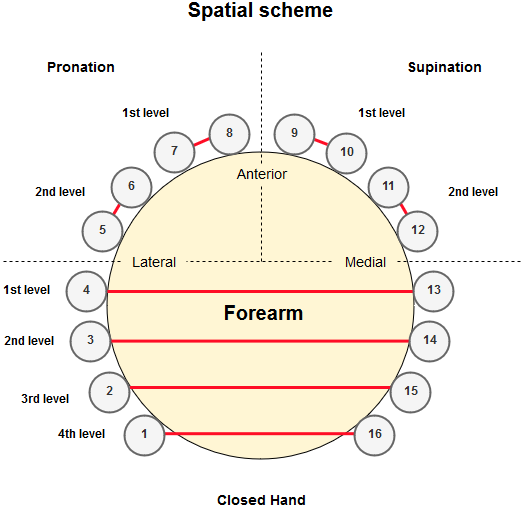
\includegraphics[width=0.48\textwidth]{figures/El_array_spatial}}
	\subfigure[Illustration of the amplitude scheme.]
	{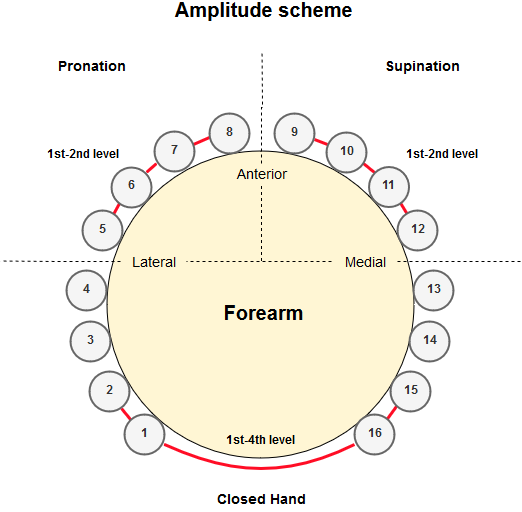
\includegraphics[width=0.48\textwidth]{figures/El_array_amplitude}}
	\caption{Figure (a) shows the spatial scheme, which is based on different pads being activated depending on the level of the grid square the cursor is located in. The highest number of possibly activated pads is four at a time. Figure (b) shows the amplitude scheme. Here, the amplitude of the active pads will increase with the increase of the level of the target location. The highest number of possibly activated pads is eight at a time.}
	\label{fig:sensconfigs}
\end{figure}


The arrows in the upper right corner of \figref{fig:gridmap} represent the hand movements needed to be performed to move the cursor in the corresponding direction. The control system will only respond to single DOF movements. Thus, the cursor is only able to move along one axis at a time and not diagonally. The subject will control the cursor with the dominant arm through an EMG electrode armband. The subject will receive stimulation from an electrode consisting of 16 electrode pads placed around the contra-lateral forearm (see illustration in \figref{fig:sensconfigs}).



\begin{figure}[H]                 
	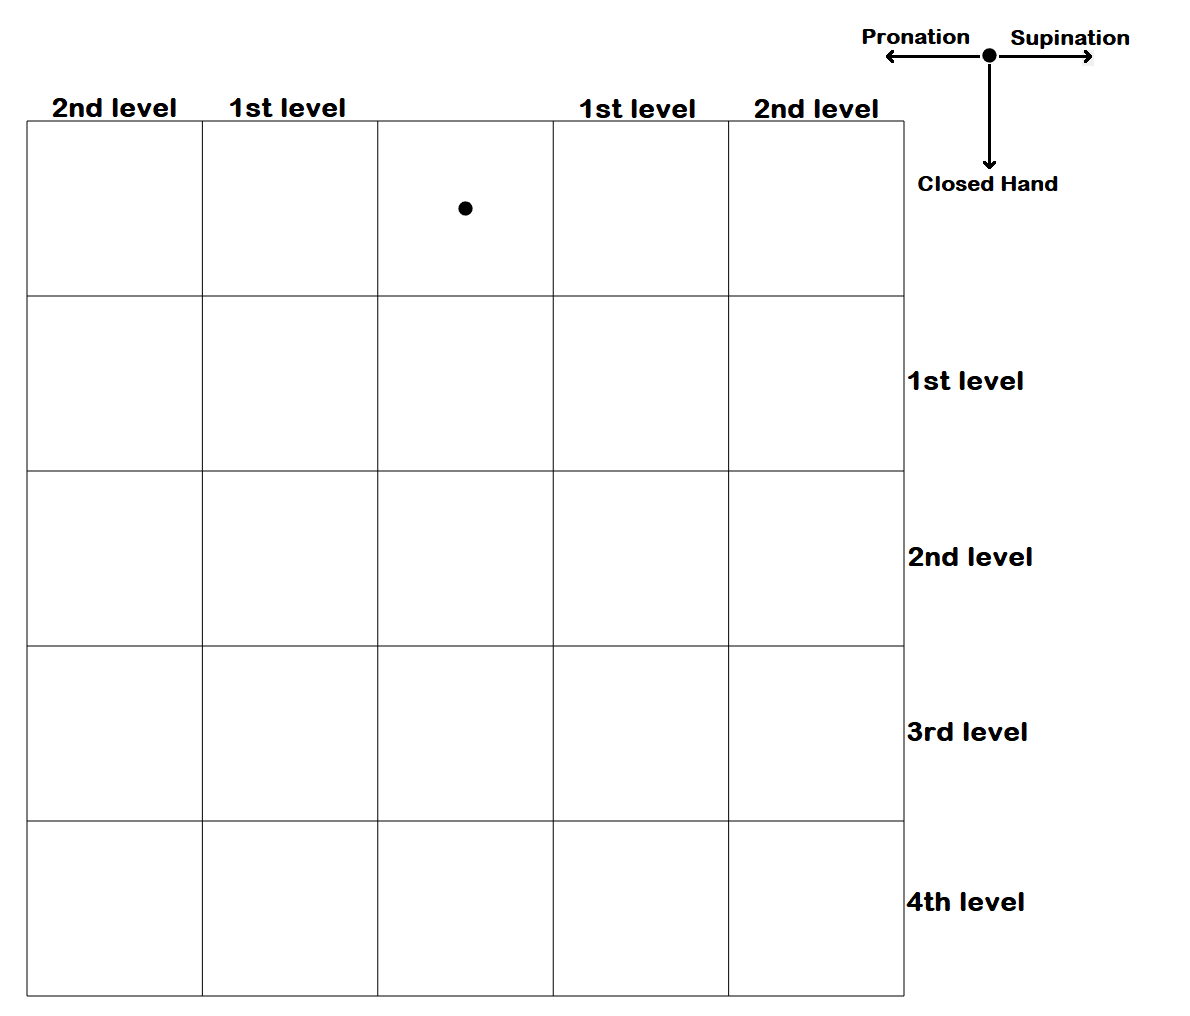
\includegraphics[width=0.9\textwidth]{figures/gridmap2}  
	\caption{Image of the grid map and cursor used in the experiment. Performing supination moves the cursor the right, pronation moves it to the left and closing the hand moves it down. Opening the hand moves the cursor up, and is used as a correction movement if a wrong movement has been made.}
	\label{fig:gridmap} 
\end{figure}
\newpage

\textbf{{\Large Hand Movements Used for Prosthetic Control}} \\

\begin{figure}[H]                 
	\includegraphics[width=0.6\textwidth]{figures/handmovements}
	\caption{Image of the hand movements used in the experiment for myoelectric prosthetic control. From top left corner: Wrist pronation, wrist supination, opened hand and closed hand.}
	\label{fig:handmovements} 
\end{figure}

\textbf{{\Large Experiment Procedure}} \\
\newline
Before the final evaluation test is carried out the subject will be trained in controlling the cursor via EMG signals, trained in interpreting the sensory feedback and trained in interpreting the sensory feedback while controlling the cursor. The evaluation test is a target reaching test, where the subject needs to move the cursor to a highlighted target consisting of one of the grid squares. The cursor will not be visible, thus, the subject will have to only rely on the information received from the sensory feedback. \\
During the experiment the subject must let the dominant arm hang relaxed down the side of the torso and the contra-lateral arm placed on a table without putting pressure on the stimulation electrode, as seen in \figref{fig:setup}. The subject must be seated during all procedures. The following order represent the chronology of the procedures the subject needs to undergo; the steps will be divided in solely control, solely sensory feedback and feedback with control. 


\textbf{{Control}} \\
\vspace{-25pt}
\begin{enumerate}
	\item Record EMG signals needed to build the prosthetic control system. To do this the subject must first perform  five movements used as reference signals: 15 seconds rest, 15 seconds prolonged maximum voluntary contraction (pMVC) of wrist supination, 15 seconds pMVC of wrist pronation, 15 seconds pMVC of opened hand and 15 seconds pMVC of closed hand. Between each contraction the subject will get a 15 seconds break to avoid fatigue. Secondly, the subject must perform movements from which the recorded signals are used to build the control system. Here, the subject controls a cursor as seen in \figref{fig:trapezoid}, and must match the cursor with trapezoidal trajectory. The cursor moves horizontally with time and the subject control the contraction intensity vertically. The subject must perform three contractions per movement: 40 \%, 50 \% and 70 \% of the pMVC. The plateau of the trapezoidal trajectory corresponds to the designated fraction. Between each performed movement, the subject gets a 15 seconds break to avoid fatigue. Lastly, a 15 seconds rest is recorded. 
	\item Train the subject's ability to control the cursor via letting the subject move freely around inside the grid map for three minutes.
	\item Train the subject's ability to control the cursor via letting the subject move freely around inside the grid map for three minutes. In this training, the cursor will not be visible, but the square the cursor is inside will be highlighted in blue. This cursor representation will be used in the remaining trainings and tests.
	\item Perform target reaching test to evaluate the subject's ability to control the cursor. The designated target will be one of the squares in the grid highlighted in red. To reach a target the blue cursor square must match the target and dwell inside it for 1.5 seconds. Then a bell sound will occur and a new target appears. The time limit for reaching a target is 30 seconds. The starting point is always the resting state square (first square in third column), and the cursor will, thus, return to starting point when a target is reached or then the time limit is reached. A total of 24 targets will appear before this test is through.
\end{enumerate}

\begin{figure}[H]                 
	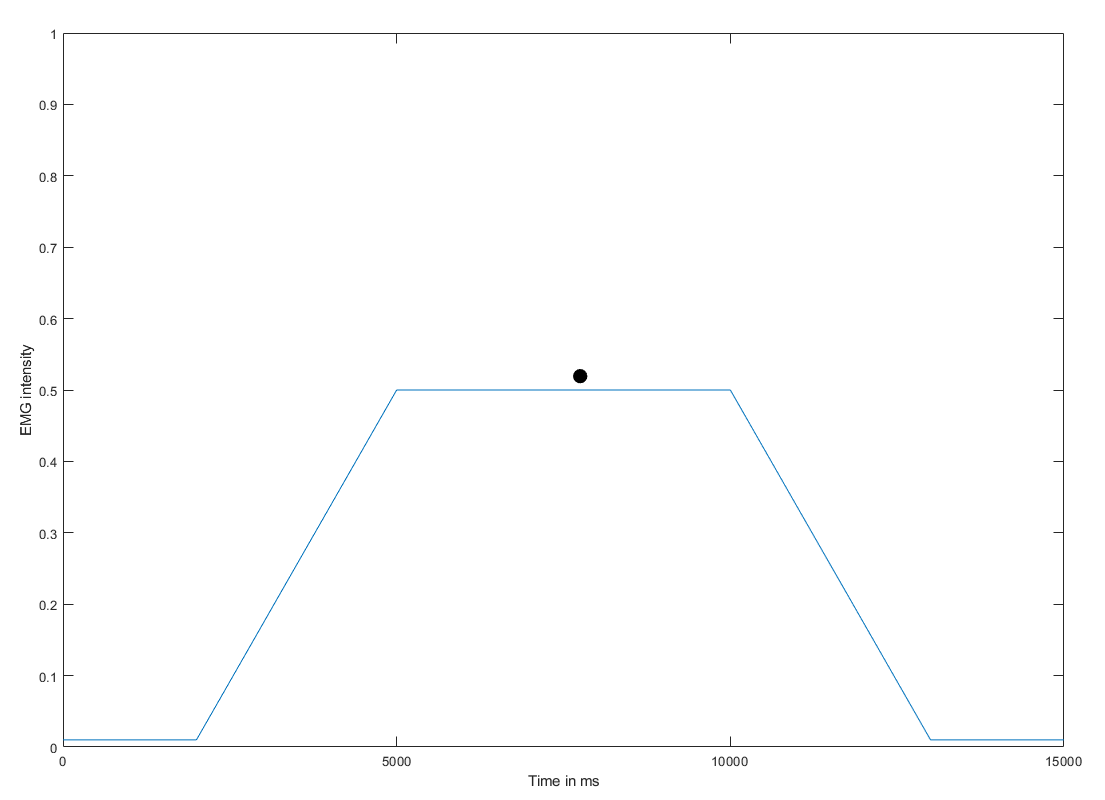
\includegraphics[width=0.65\textwidth]{figures/trapezoid2}  
	\caption{Image of the trapezoidal trajectory used when recording EMG signals used to build the control system. The subject controls the black cursor in height by increasing contraction intensity.}
	\label{fig:trapezoid} 
\end{figure}

\textbf{Sensory Feedback} \\
\vspace{-25pt}
\begin{enumerate}
	\item Record current amplitude thresholds needed to build the sensory feedback schemes. For each electrode the subject must first note when the stimulus is felt clearly. When all thresholds are set, the sensation of neighbouring electrodes are compared to ensure homogeneity in the sensation. Afterwards the same procedure is performed for the subject's tolerance threshold. 
	\item Train the subject's ability to interpret sensory feedback for one of the schemes. This is done by exposing the subject to feedback from 12 grid squares. The subject will experience the transitions from square to square until the designated square is reached. The path taken to reach the designated square is the direct route (full length in one direction and then the other), but which direction that will be travelled first is predetermined by the investigators.
	\item Perform reinforcement learning on all grid squares. The path taken to reach the designated square is the direct route, but which direction that will be travelled first is predetermined by the investigators. During this step the subject must look away from the computer screen. When a designated square is reached, the subject will be asked where the cursor is located. After answering the subject will be informed on whether is was correct, and told the correct location, if the answer was incorrect. 
	\item Repeat reinforcement learning from step 3. The order of the squares and the route to each square will vary from step 3.
\end{enumerate}

\textbf{Sensory Feedback with Control} \\
\vspace{-25pt}
\begin{enumerate}
	\item Train the subject's ability to control the cursor while receiving sensory feedback via letting the subject move freely around inside the grid map for three minutes.
	\item Perform target reaching test where the cursor is invisible to evaluate how well the subject can utilize the sensory feedback regarding the cursor location. This test has the same format as the target reaching test from the control procedure step 3.
	\item Repeat target reaching test from step 2.
	\item Redo sensory feedback steps and sensory feedback with control steps with sensory feedback from the remaining scheme.
\end{enumerate}


\newpage
\textbf{{\Large Experiment Setup}} \\

\begin{figure}[H]                 
	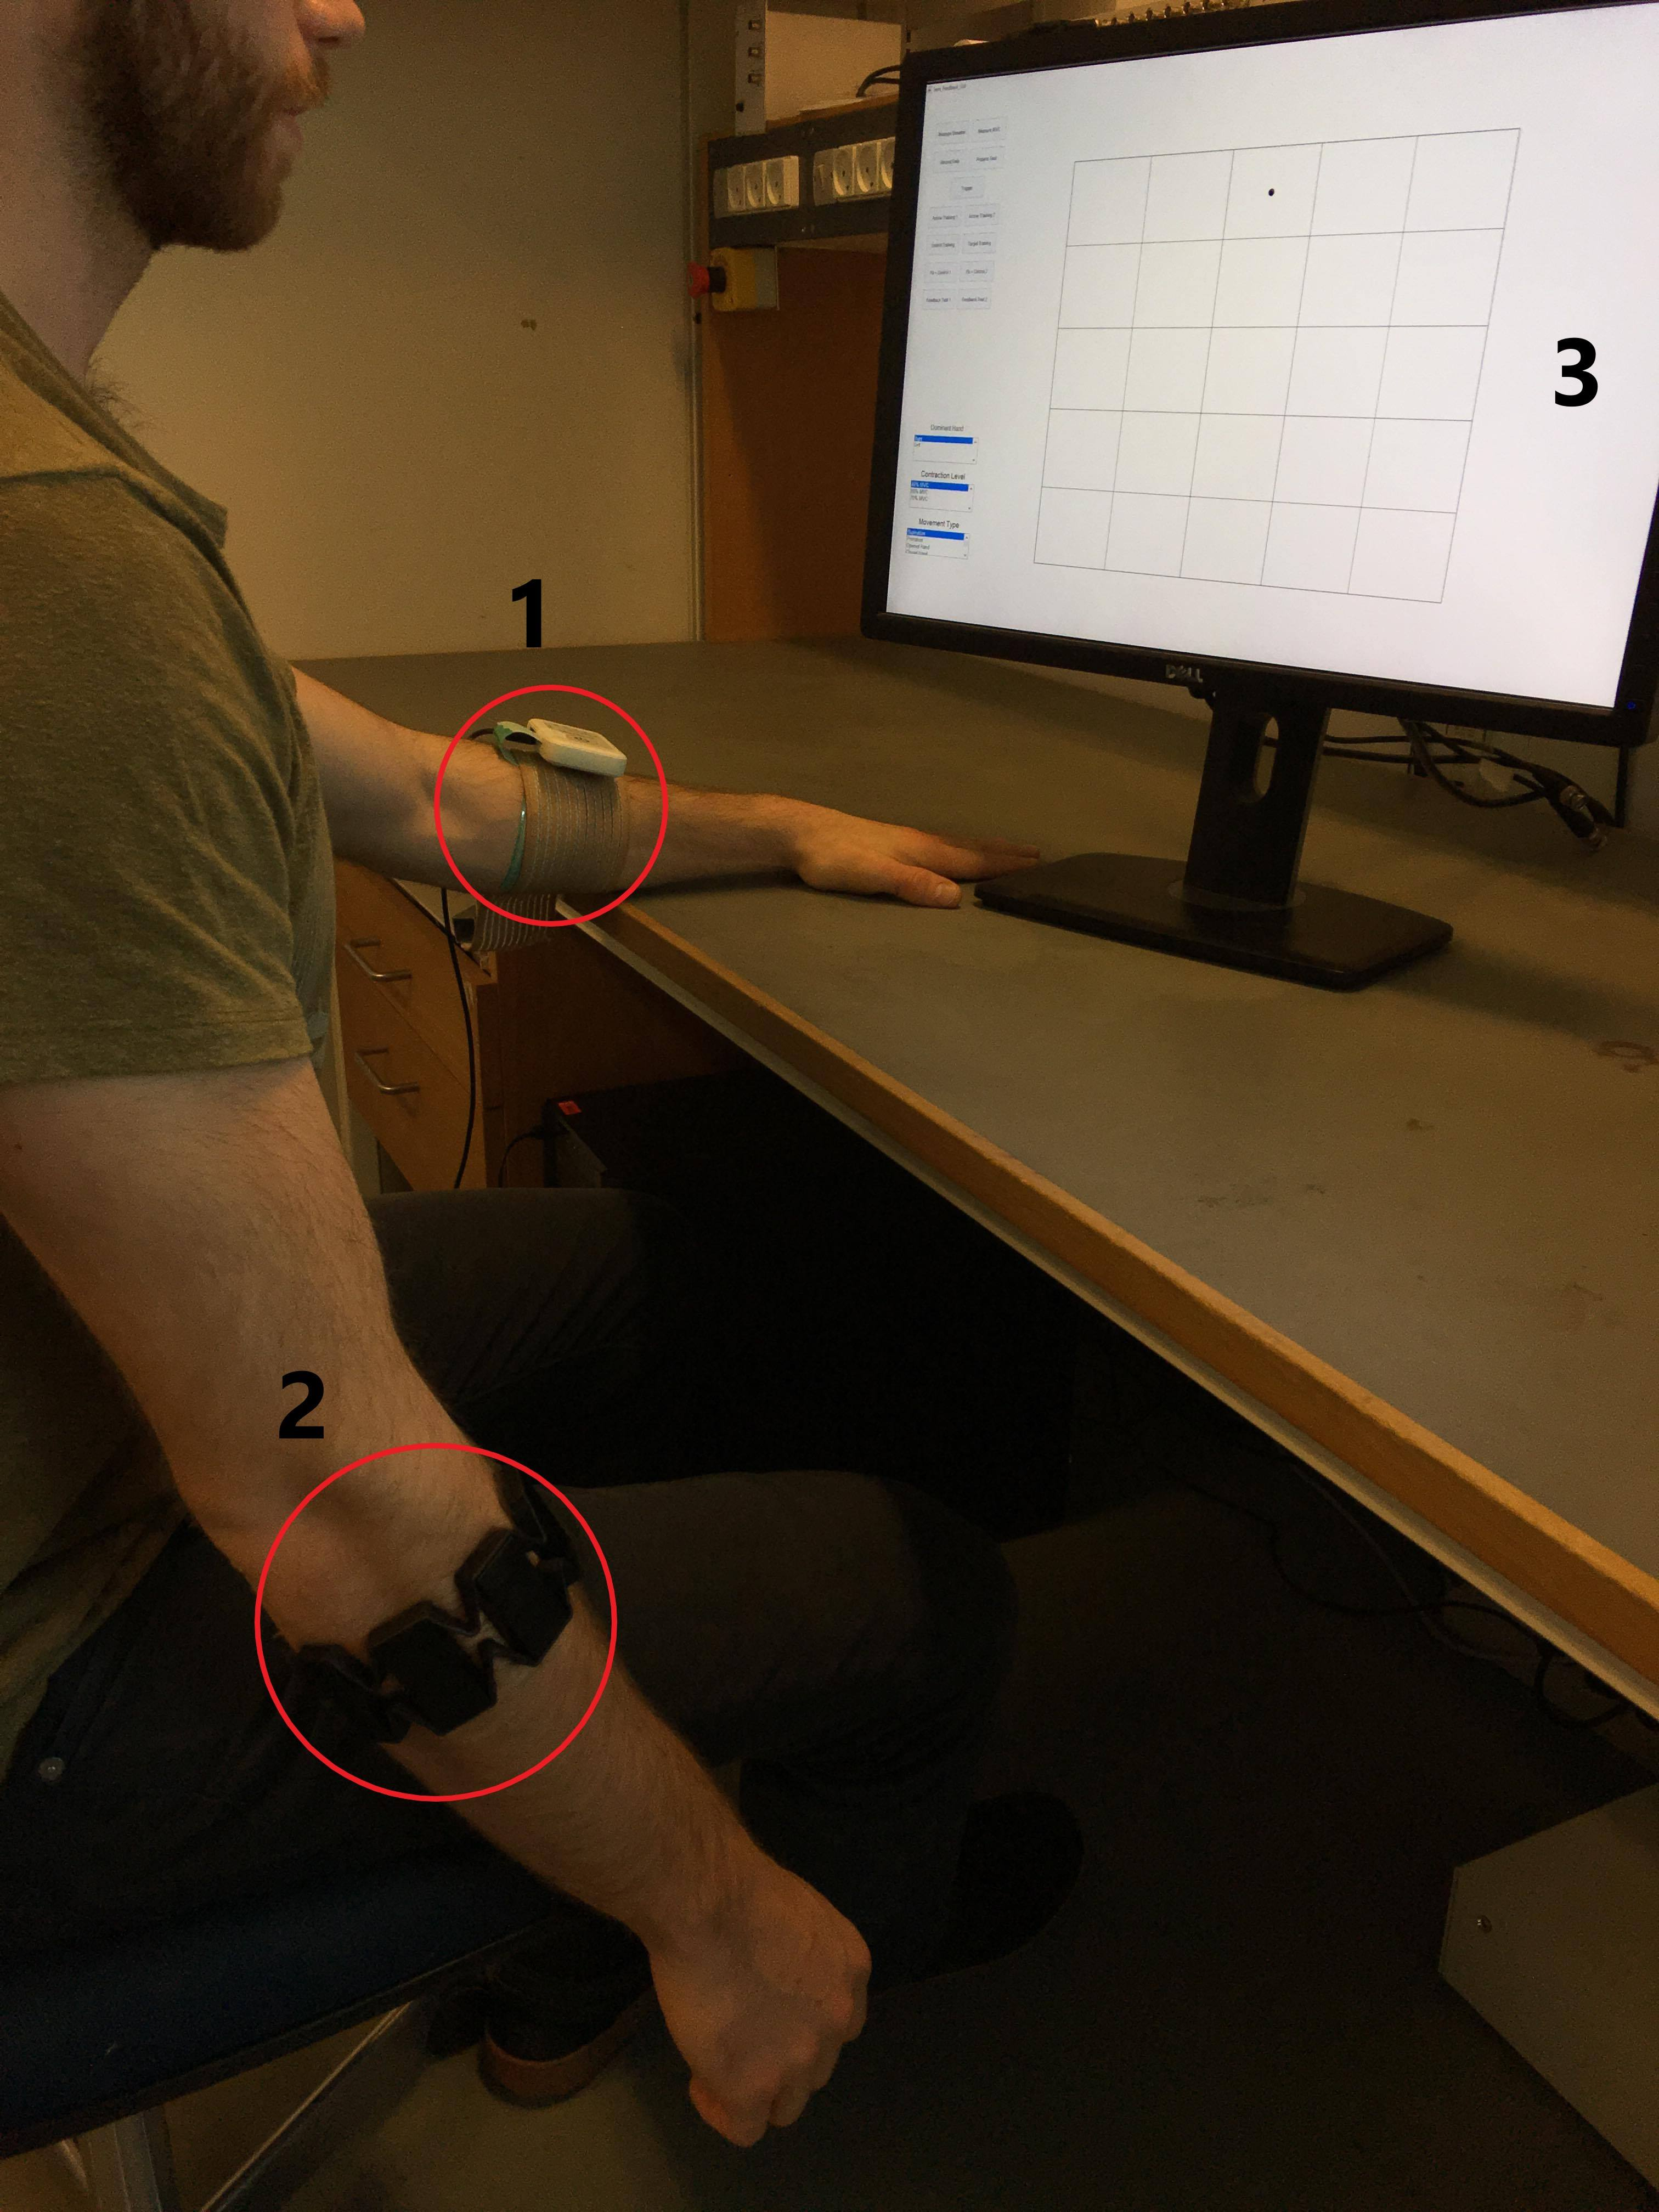
\includegraphics[width=0.8\textwidth]{figures/setupimg}  
	\caption{Image of the experimental setup. 1) is the stimulation device with the stimulation electrode placed under the brown armband, 2) is the electrode armband used to record EMG signals and 3) is the computer screen used to guide the subject and display tasks.} 
	\label{fig:setup} 
\end{figure}


%\newpage
\section{Short Experiment Description} \label{SED}

\textbf{Project Title} \\
Evaluation of Electrotactile Feedback Schemes in
Combination with Myoelectric Control.

\textbf{Experiment Purpose} \\
When a person gets amputated on the lower arm, he/she can receive a functional prosthesis. This is controlled by muscle signals from the user, where the muscle signals are translated into a prosthesis movement. However, many functional prostheses do not provide sensory feedback, which results in some users to abandon their prosthesis.\\
The purpose of the experiment is to compare how subjects perform in an evaluation test when receiving feedback from two different electrical stimulation configurations, while controlling a virtual prosthesis. The results might provide information on which feedback that seems more intuitive to use in a real prosthesis.   

\textbf{Experiment Overview} \\
The experiment will take place in the laboratory D3-107 at Aalborg University. The duration of the experiment is estimated to be 2 hours and 30 minutes. \\
During the experiment a myoelectric armband will be placed on the dominant forearm and used to record muscle activity while the subject performs four different hand gestures. Subsequently, an evaluation of the ability to reproduce the gestures will be made. \\
Afterwards, an electrode armband capable of delivering electrical stimulation at 16 different locations will be placed on the non-dominant arm. The subject will determine the level of sensory perception and tolerance level. The subject will then be made familiar with and trained in understanding two different feedback configurations that represents the possible states the virtual prosthesis can be in. At the end, an evaluation of the subject’s ability to understand the feedback while making the trained hand gestures will be made. \\
At the day of the experiment, please refrain from using any types of sensory deprivation drugs (painkillers and alike). The test subject will not receive monetary compensation after the experiment. 

\end{appendices}


\end{document}
